\documentclass[12pt,titlepage,oneside]{memoir}
\usepackage{graphicx}
\usepackage{amsmath}
\usepackage{amsfonts}
\usepackage{amssymb}
\usepackage{hyperref}


\chapterstyle{southhall}
\newcommand{\HRule}{\rule{\linewidth}{0.5mm}}
\pagestyle{plain}
\setstocksize{11in}{8.5in}
\settrimmedsize{11in}{8.5in}{*}
\settrims{0in}{0in}
\settypeblocksize{8.5in}{35pc}{*}
\setlrmargins{1in}{*}{*}
\setulmargins{1in}{*}{*}
\setheadfoot{13pt}{26pt}
\setheaderspaces{*}{13pt}{*}
\checkandfixthelayout


\begin{document}
\begin{titlingpage}
\begin{center}


\vspace{50mm}
% Title
\HRule \\[0.4cm]
{ \huge \bfseries Razbot Build Instructions}\\[0.4cm]

\HRule \\[1.5cm]

% Author and supervisor
\begin{minipage}{0.4\textwidth}
\begin{flushleft} \large
\emph{Author:}\\
Robbie \textsc{Edwards}\\
\end{flushleft}
\end{minipage}
\vfill
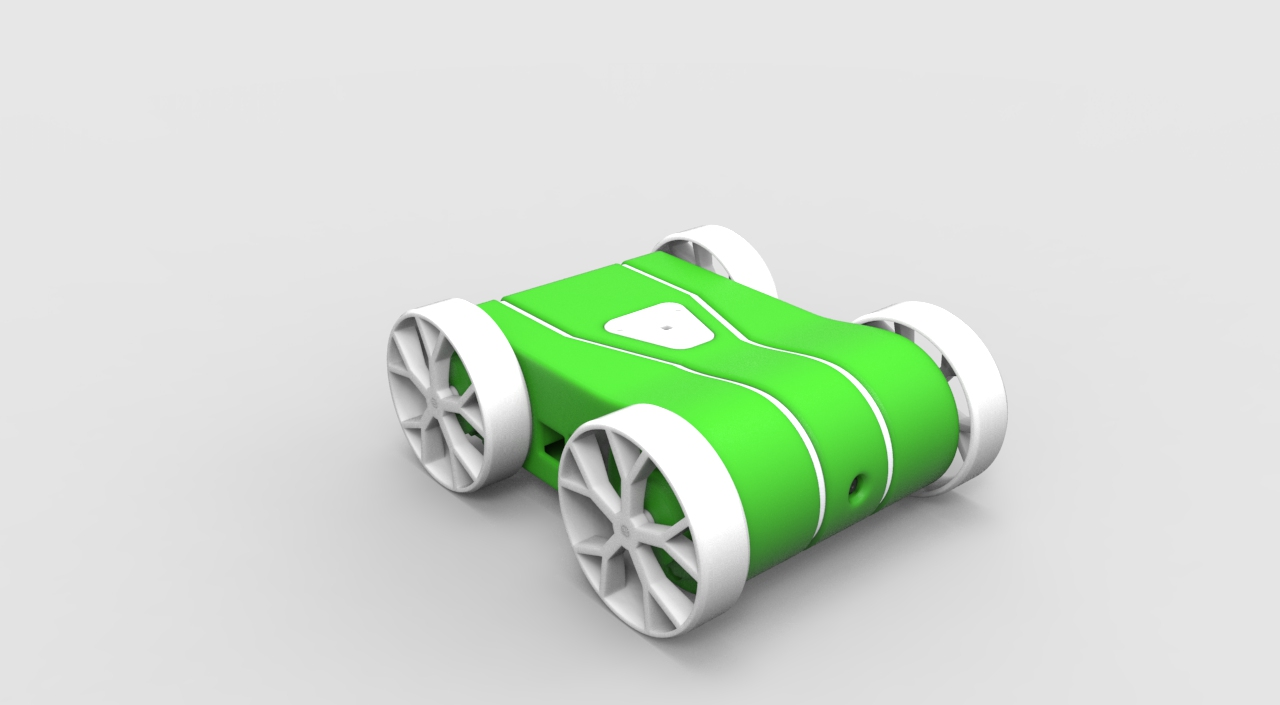
\includegraphics[width=450px]{render/pibot2.jpg}
\vspace*{1cm}

% Bottom of the page
{\large \today}

\end{center}
\end{titlingpage}


%\frontmatter
%\tableofcontents

\mainmatter
\counterwithout{figure}{chapter}
%\section{Introduction}
%This document presents a brief overview of some of the many personal and academic projects carried out by Robbie Edwards. Further documentation is available upon request for the listed projects or on any of the work related or artistic projects not shown here. 

\chapter{Overview}
%\begin{figure}[!ht]
%\includegraphics[width=500px]{pawly.pdf}
%\centering
%\end{figure}

The Razbot was created to provide a low cost Linux/Robot Operating System (ROS) enabled mobile robot platform. The goal was to provide access to high quality software on a low cost platform which can be printed and assembled by the user. It currently runs ROS Indigo and Raspbian Jessie. The \href{http://wiki.ros.org/ROS/Introduction}{Robot Operating System} is a BSD licensed meta-operating system which provides a convenient set of tools for developing software for robot applications. It is well documented online and explained in further detail in various \href{http://wiki.ros.org/Books}{books}. Many open source ROS packages are freely available to carry out robot related software tasks ranging from interfacing with sensor hardware to carrying out navigation and mapping \\

\section{Features}:
\begin{itemize}
\item Raspberry Pi with Raspbian Jessie
\item ROS Indigo
\item Independent Motor Control of each wheel
\item WS2812b Status LED
\item Raspberry Pi camera
\item Lithium Battery: Turnigy Nanotech 3S 2200mAh,
\item 2 hour or greater run time
\item USB ports, Wifi
\item Logitech F710 Game pad expandable
\end{itemize}

\pagebreak
\begin{figure}[!htbp]
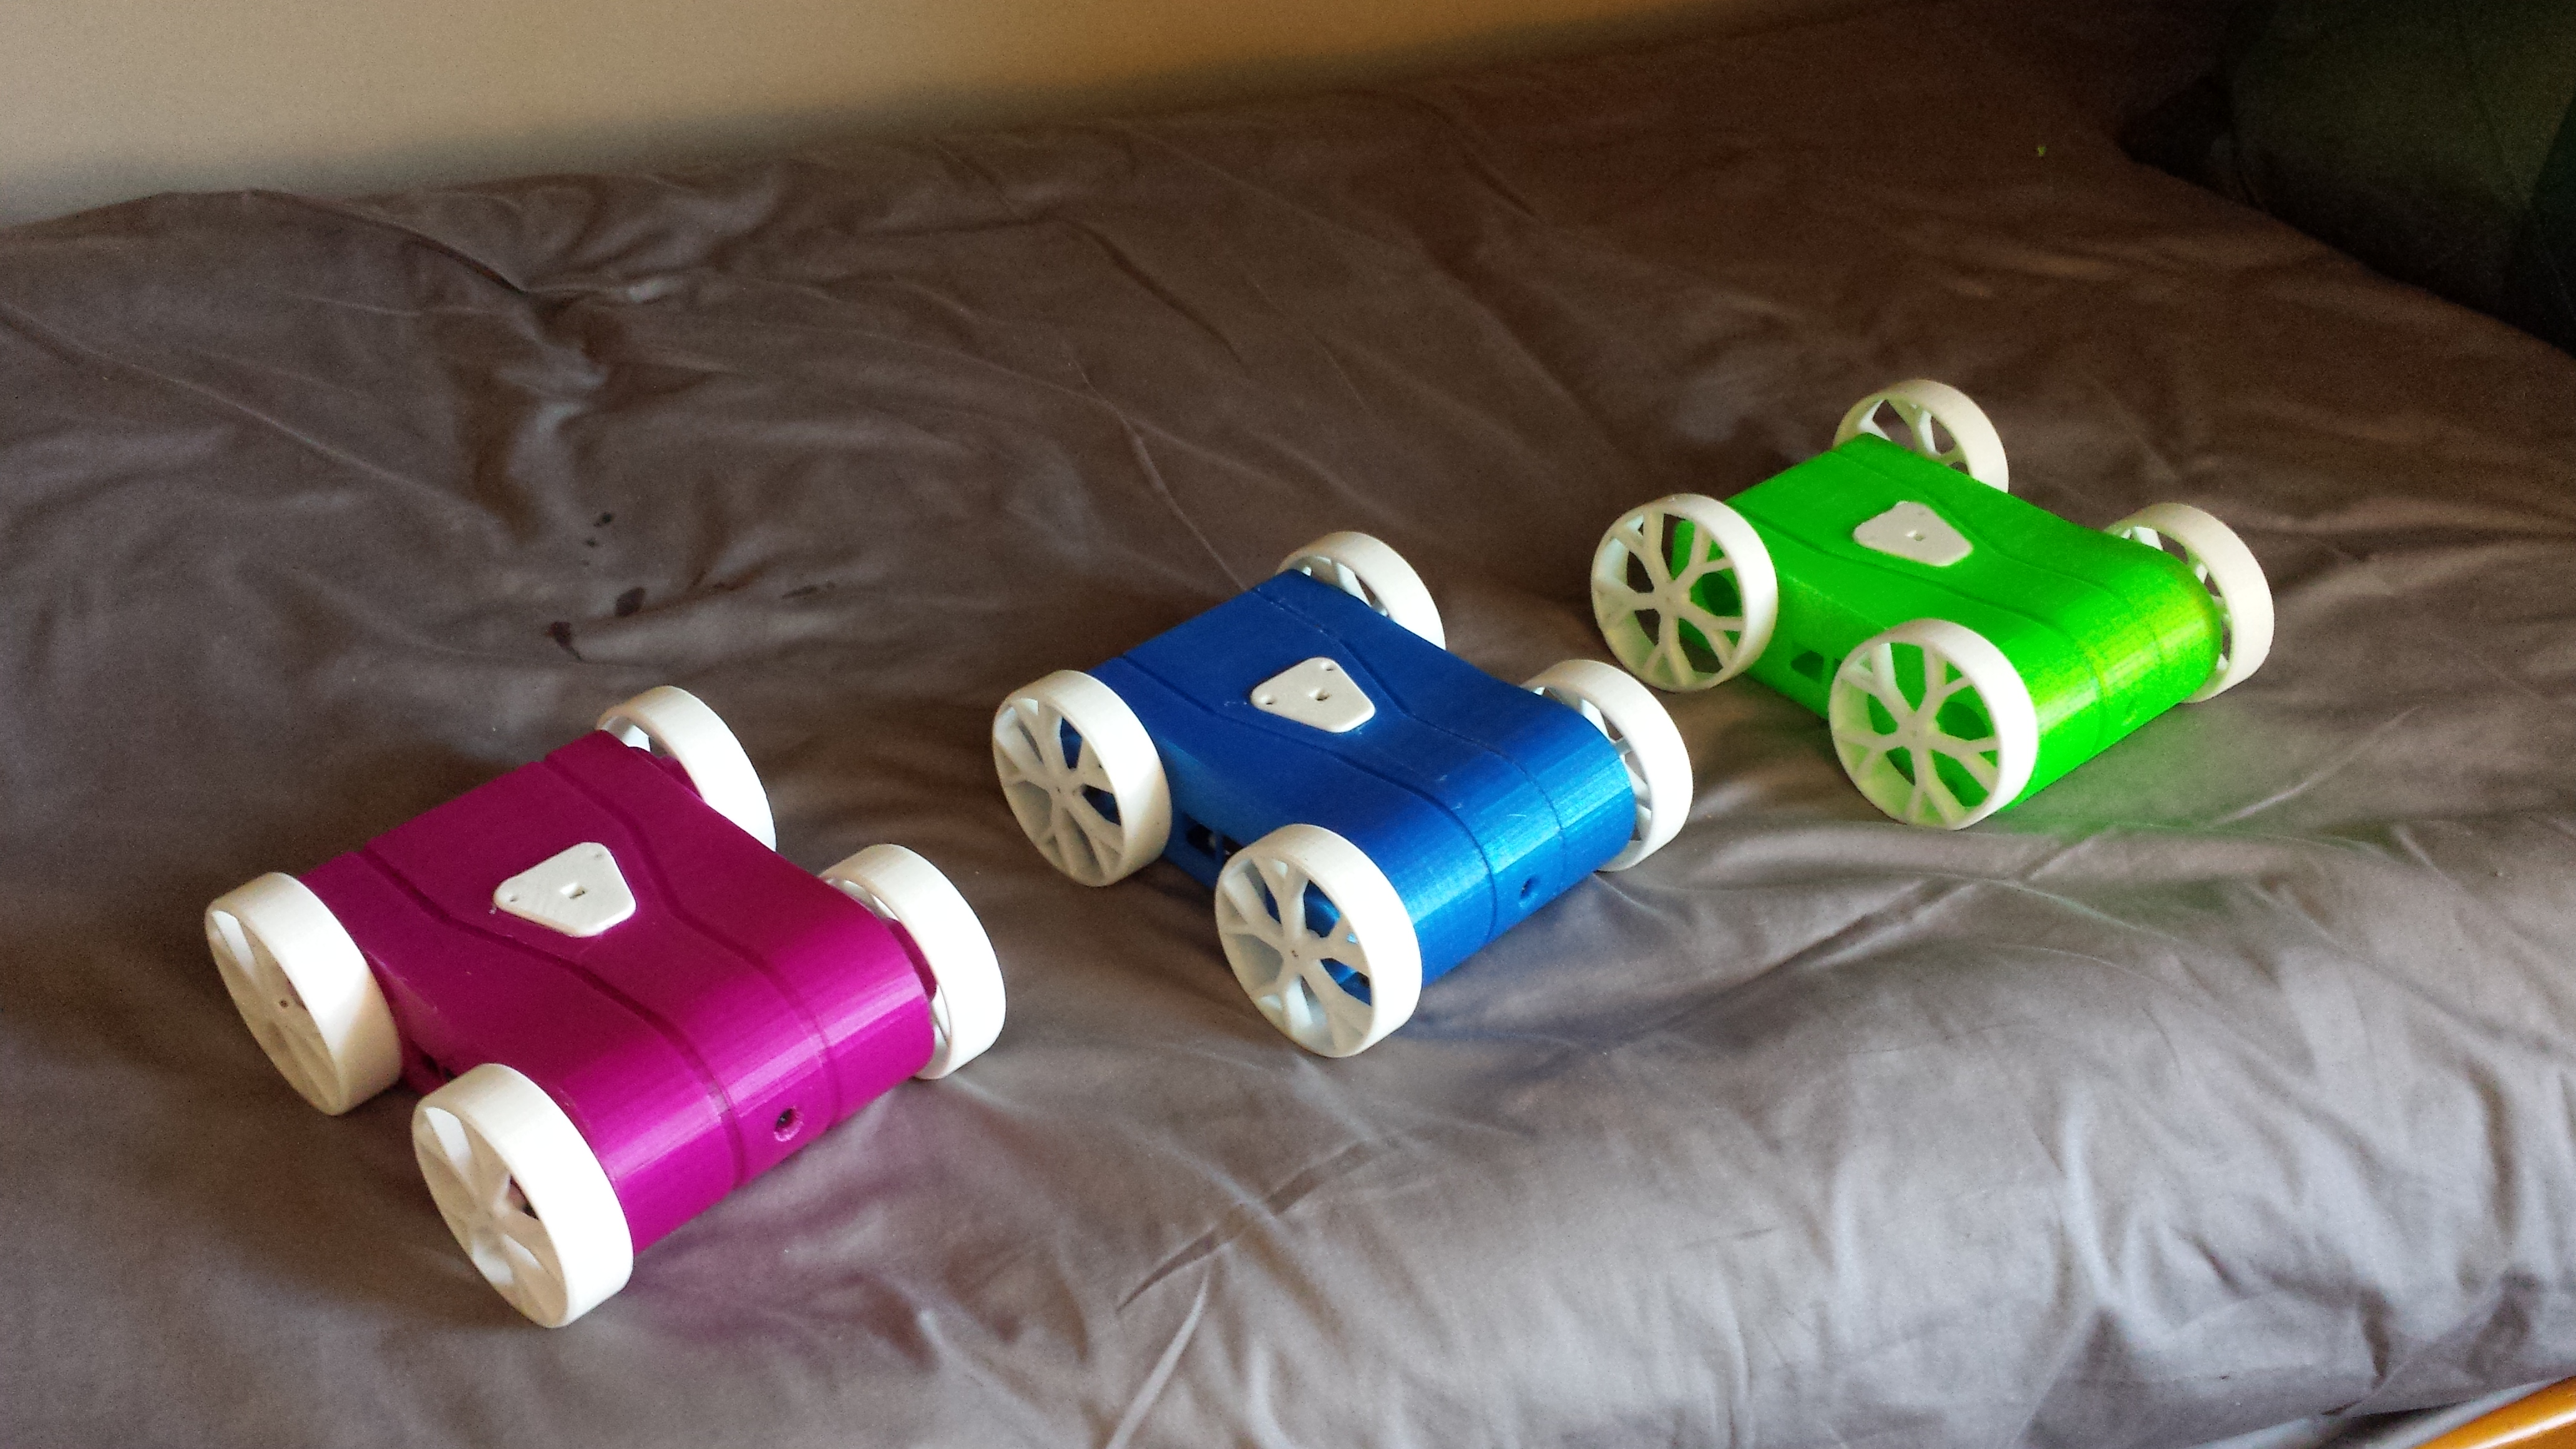
\includegraphics[width=350px]{picture/3bots.jpg}
\centering
\end{figure}


\begin{figure}[!htbp]
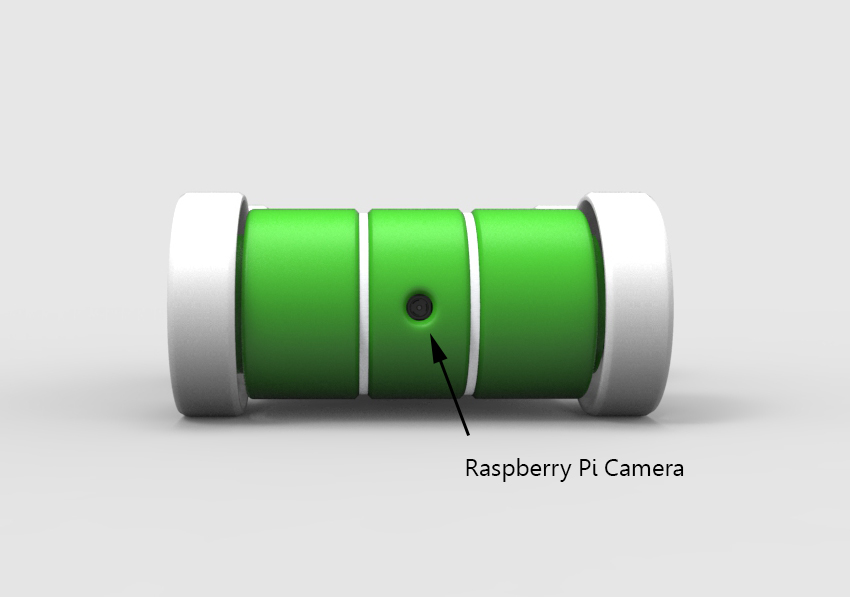
\includegraphics[width=350px]{render/pibotfront.jpg}
\centering
\end{figure}

\begin{figure}[!htbp]
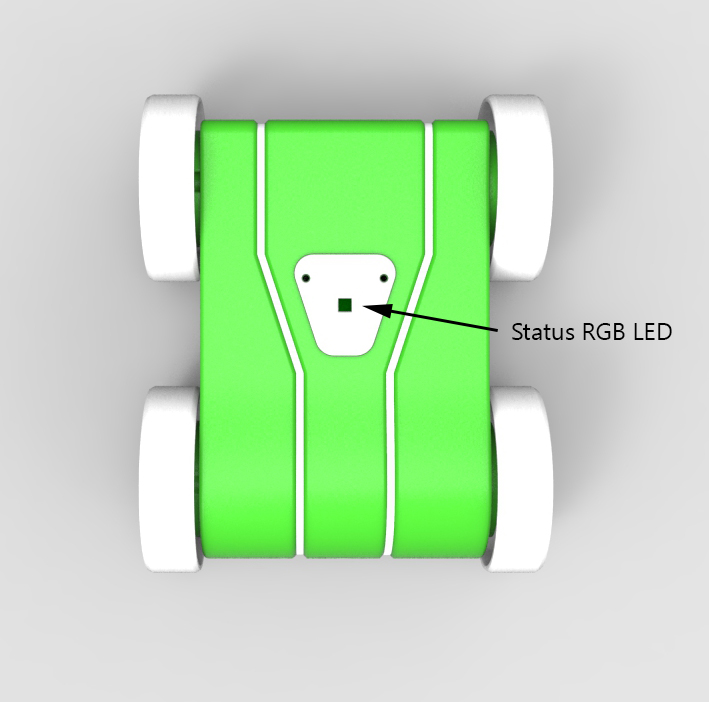
\includegraphics[width=350px]{render/pibottop.jpg}
\centering
\end{figure}

\begin{figure}[!htbp]
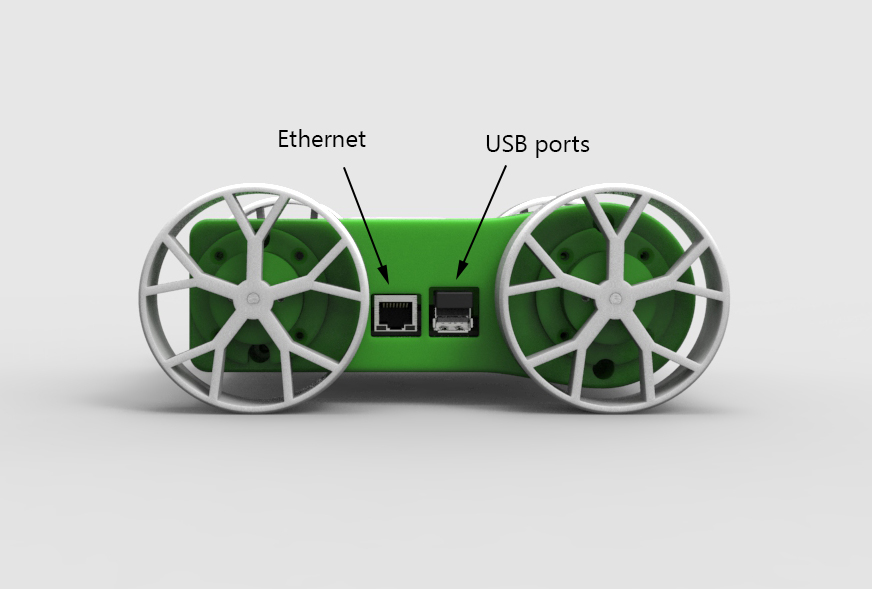
\includegraphics[width=350px]{render/pibotstarboard.jpg}
\centering
\end{figure}

\begin{figure}[!htbp]
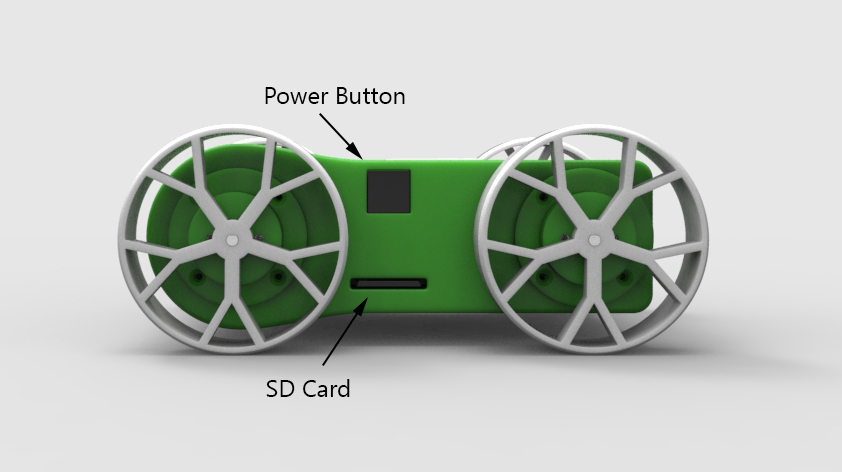
\includegraphics[width=350px]{render/pibotport.jpg}
\centering
\end{figure}

\begin{figure}[!htbp]
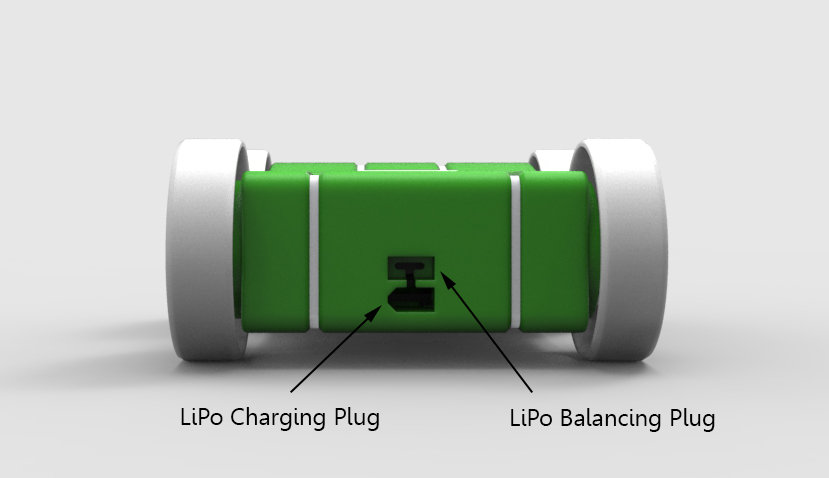
\includegraphics[width=350px]{render/pibotback.jpg}
\centering
\end{figure}

\begin{figure}[!htbp]
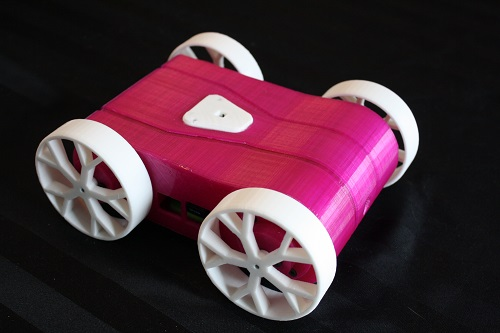
\includegraphics[width=350px]{picture/bot1.jpg}
\centering
\end{figure}

\pagebreak
\chapter{Bill of Materials and Required Tools}
\section{Parts and Tools}

The following tables provide a list of the parts and tools required to build the rover. The parts are currently sourced from many suppliers resulting in many orders and higher shipping costs. 
One day, someone can perhaps offer a single source supply for all components necessary to build the rover. Table \ref{table:BOM} lists the major components of the rover. Table \ref{table:opBOM}. The basic tools required are found in Table \ref{table:tools}. A list of screws required for assembly is found in Table \ref{table:screws}. The wiring components are in Table \ref{table:wires}. The instructions for the assembly of the circuit board and a list of the required components are given in a later section.

\begin{table}[!h]
\begin{tabular}{p{4cm} | p{3.5cm} | c | c | c}
part & supplier &  quantity &   total cost & image\\
\hline
12V 100rpm 25mm gearmotors & ebay, aliexpress, amazon&  4  & \$40 & 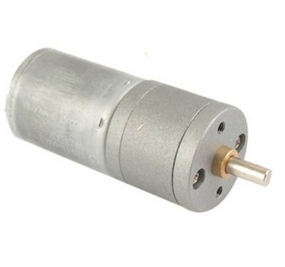
\includegraphics[width=80px]{picture/motor.png}\\
Raspberry Pi B, B+, 2 & adafruit, element14 & 1 & \$40-\$60 & 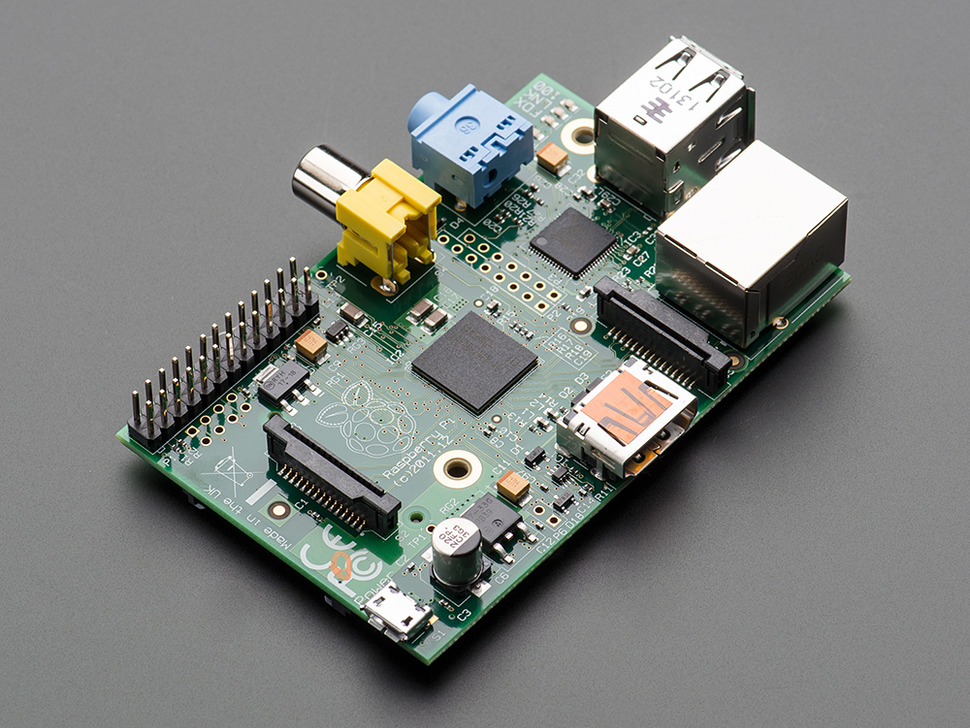
\includegraphics[width=80px]{picture/pi.jpg}\\
Raspberry Pi Wifi USB Adapter & adafruit, element14 & 1 & \$12 & 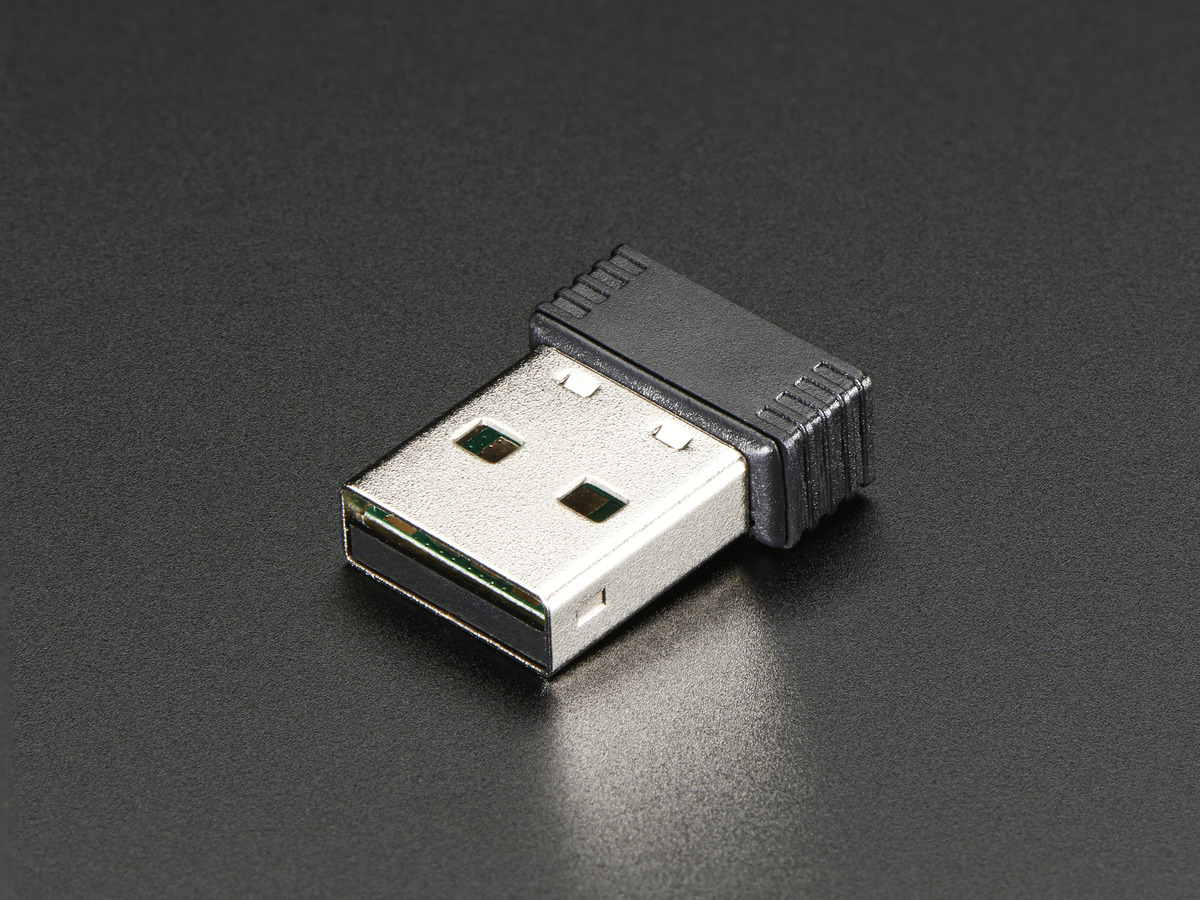
\includegraphics[width=80px]{picture/piwifi.jpg}\\
Raspberry Pi Camera Board, NoIR & adafruit, element14 & 1 & \$30 &  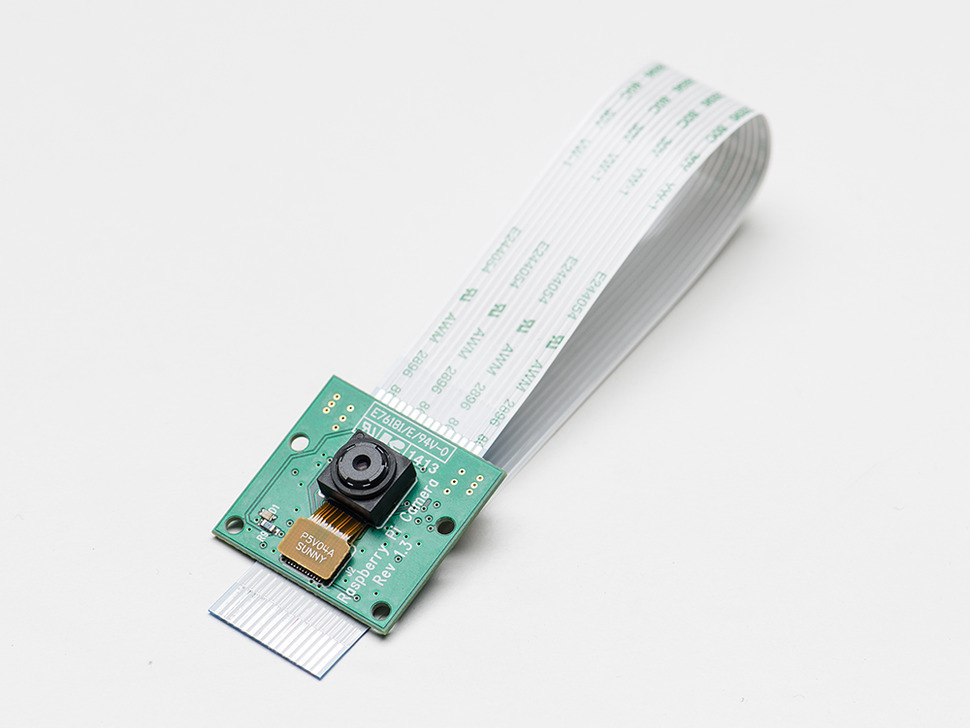
\includegraphics[width=80px]{picture/picam.jpg}\\
SD card & & 1 & \$15 & NA\\
Turnigy 2200mAh 3S 20C LiPo Pack & HobbyKing & 1 & \$10 &  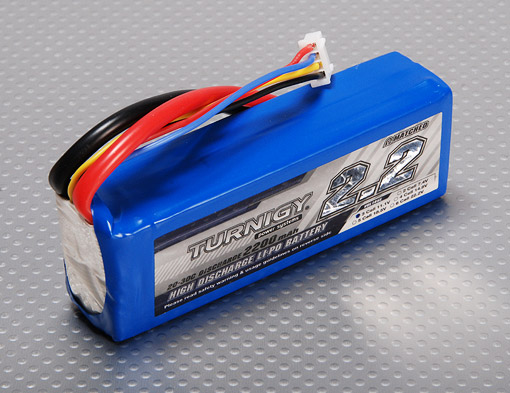
\includegraphics[width=80px]{picture/lipo.jpg}\\
Razbot Electronics Board & None & 1 & N/A &  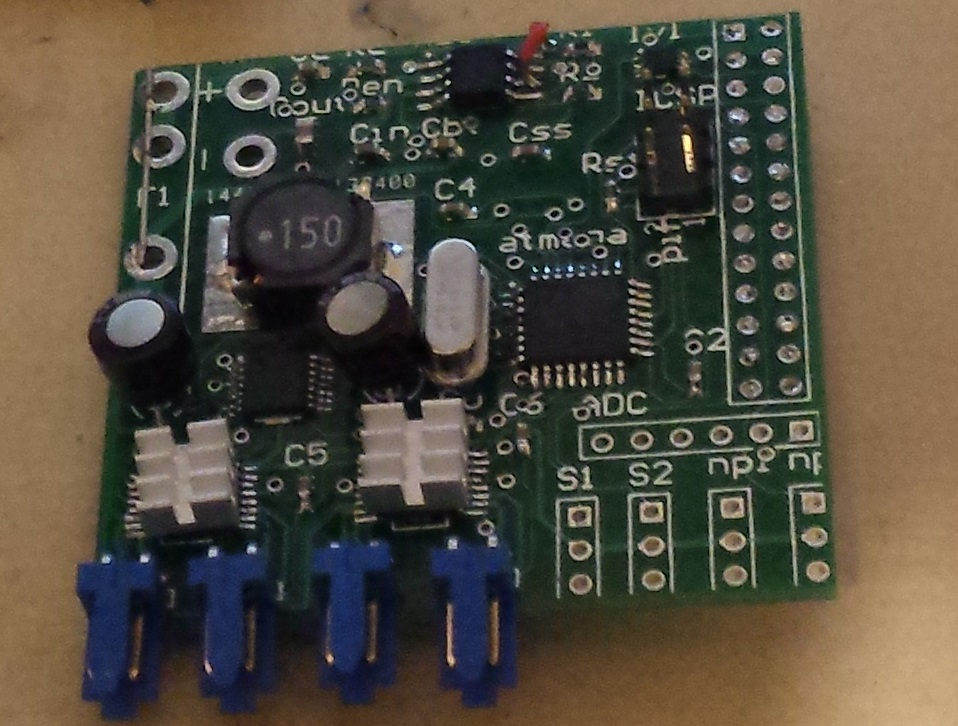
\includegraphics[width=80px]{picture/piboard.jpg}\\
Lithium Polymer B3AC Battery Charger & HobbyKing & 1 & \$8 & 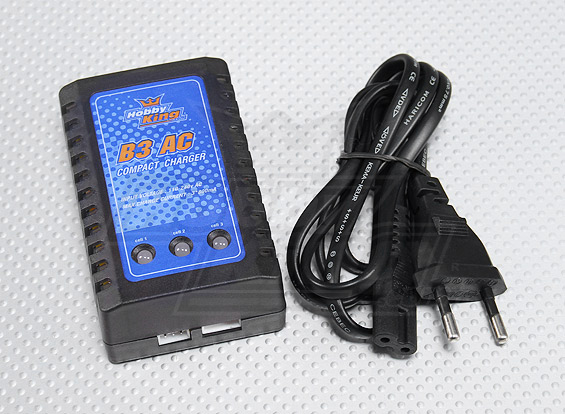
\includegraphics[width=80px]{picture/charger.jpg}\\
Wiring and connectors & NA & 1 & \$15 & NA \\
Screws and bolts & NA &1 & \$10 & NA \\
3D printed parts & NA & 12 & \$30 filament & NA \\
\end{tabular}
\caption{Major Components Bill of Materials}
\label{table:BOM}
\end{table}

\begin{table}[!h]
\begin{tabular}{p{4cm} | p{3.5cm} | c | c | c}
part & supplier &  quantity &   total cost & image\\
\hline
Logitech F710 Gamepad & Bestbuy, computer stores & 1  & \$45 & 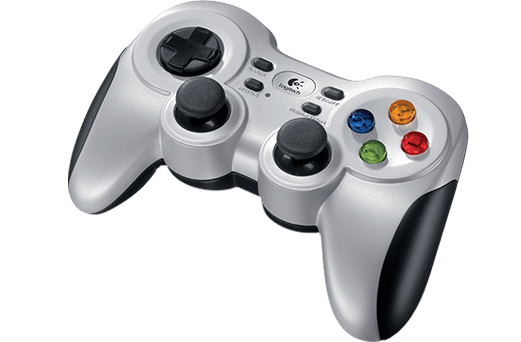
\includegraphics[width=80px]{picture/f710.png}\\
\end{tabular}
\caption{Optional Equipment}
\label{table:opBOM}
\end{table}

\begin{table}[!h]
\begin{tabular}{c | c}
\hline
recommended tools & \\
\hline
Hex key set (metric) 1.5,2,2.5,3mm sizes & 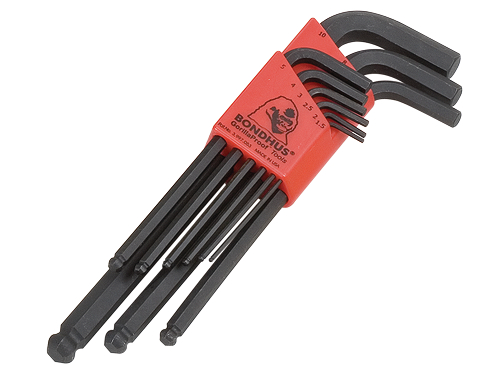
\includegraphics[width=80px]{picture/hexkey.jpg}\\
Soldering Iron with medium and fine tips & 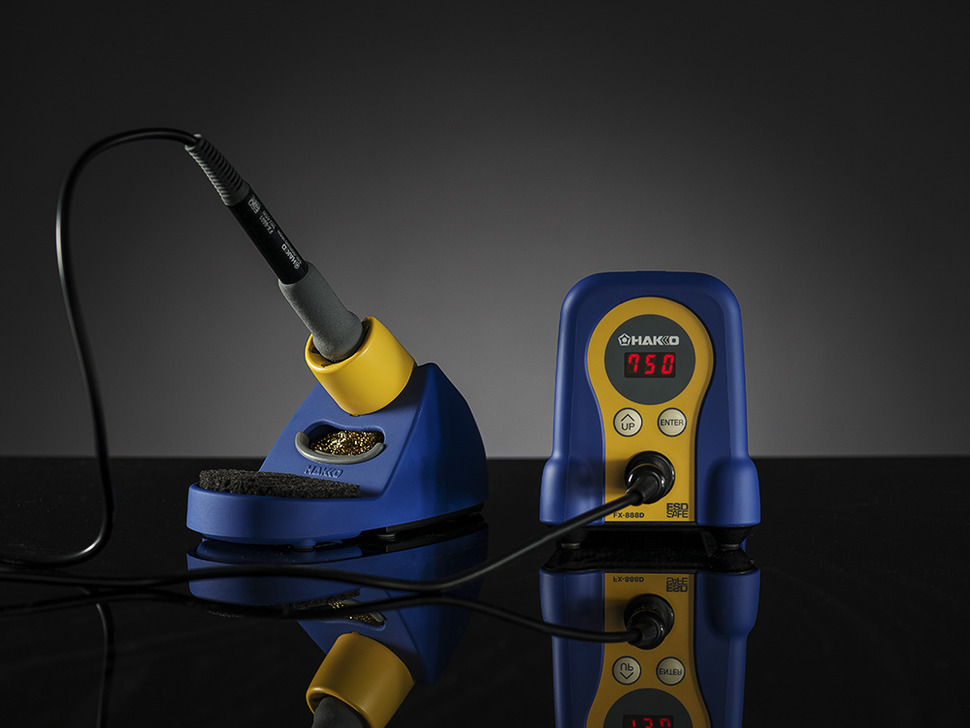
\includegraphics[width=80px]{picture/solderingiron.jpg}\\
Hobby Knife & 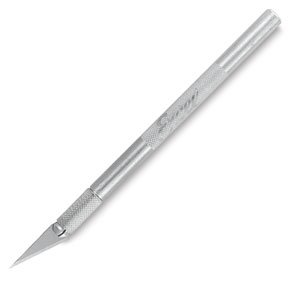
\includegraphics[width=80px]{picture/knife.jpg}\\
Wire strippers & 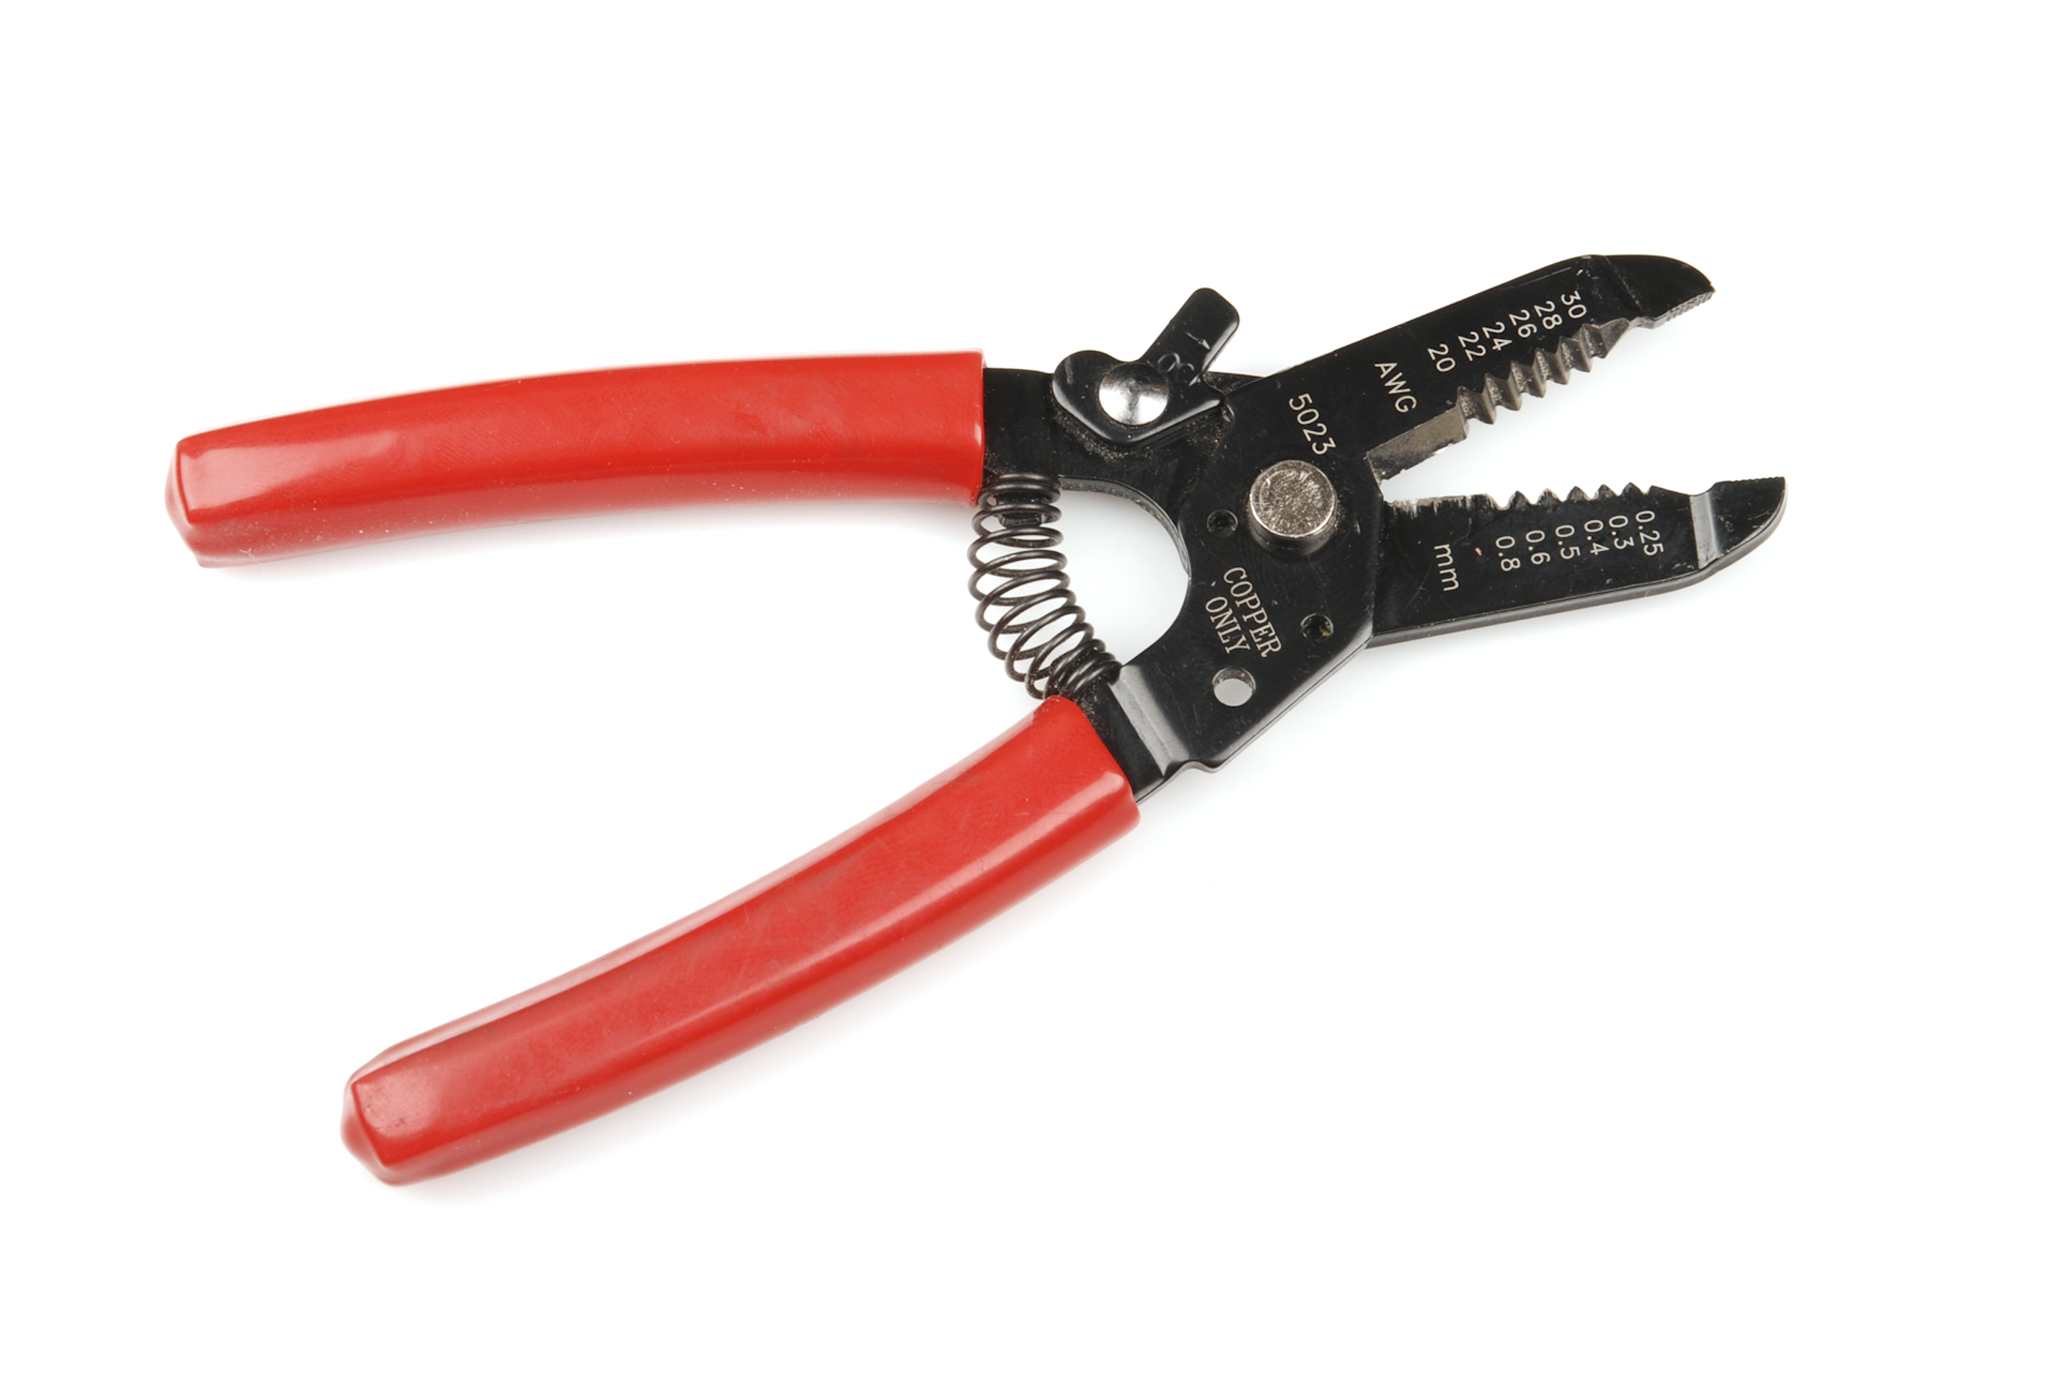
\includegraphics[width=80px]{picture/wirestripper.jpg}\\
AVR ISP mkii & 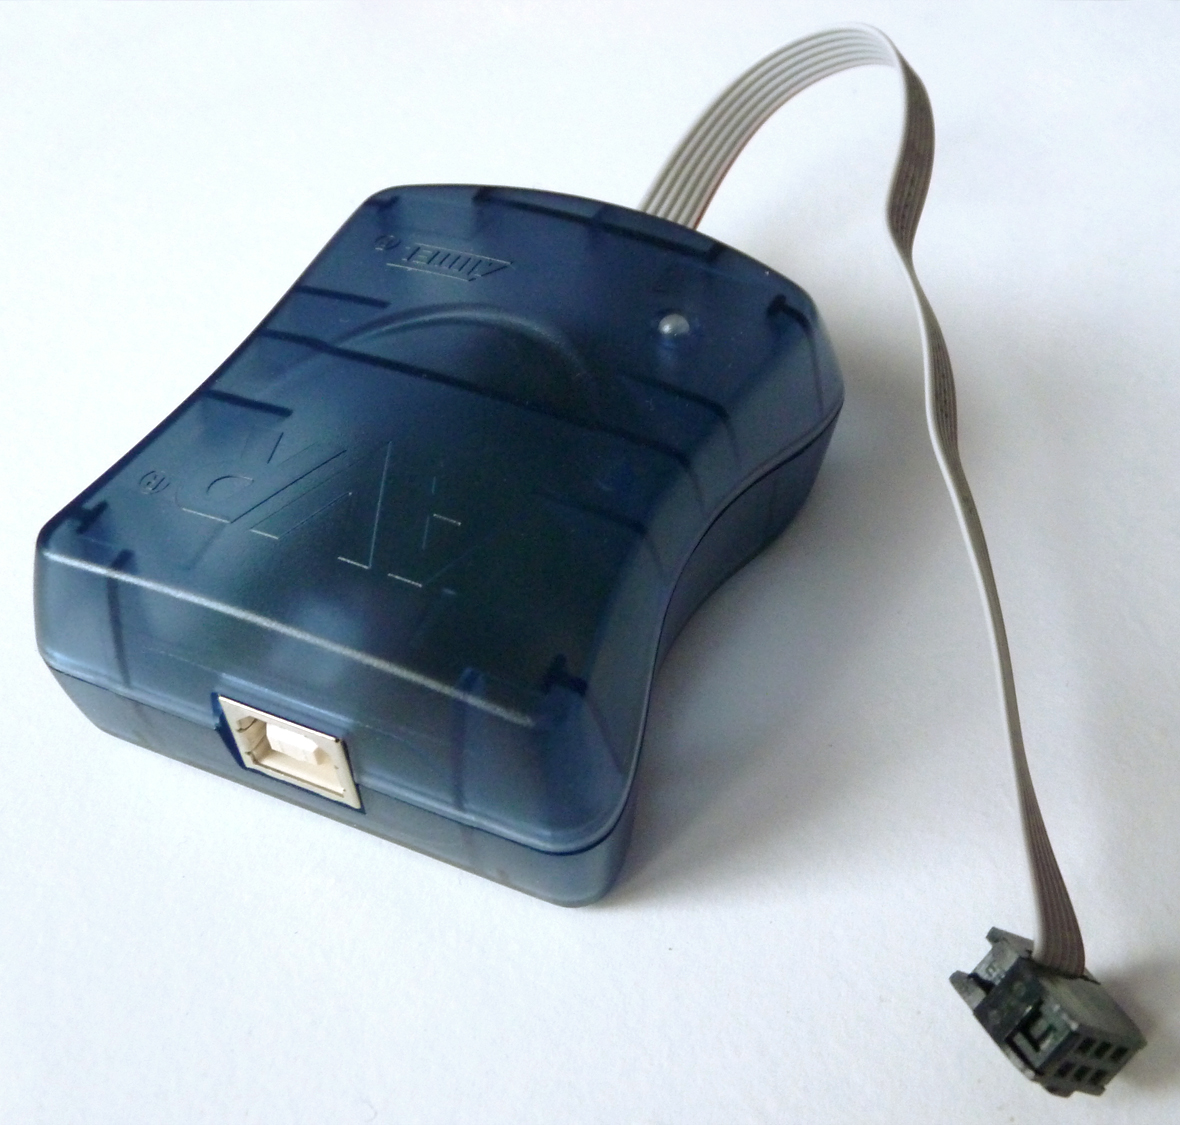
\includegraphics[width=80px]{picture/avrisp.jpg}\\
\hline
optional tools & \\
\hline
M3, M4 drill taps  & 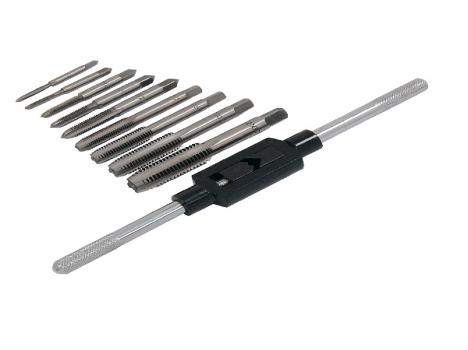
\includegraphics[width=80px]{picture/taps.jpg}\\
Hobby Tweezers & 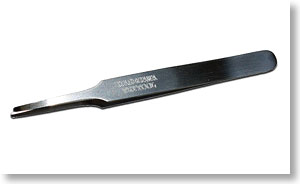
\includegraphics[width=80px]{picture/tweezer.jpg}
\end{tabular}
\caption{Recommended Tools}
\label{table:tools}
\end{table}


\begin{table}[!h]
\begin{tabular}{p{5cm} | c | c | c }
part & Spaenaur part number & quantity & image \\
\hline
Hex Socket Cap Screw M4 x 0.7mm x 25mm Full Thread & 367-022 & 4 & \\
Hex Socket Low Head Cap Screw M3 x 0.5mm x 5mm	& 366-1071 & 12 &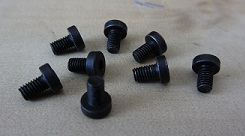
\includegraphics[width=80px]{hw/M3X06LHC.jpg} \\
Hex Socket Flat Head Cap Screw M3 x 0.5mm x 10mm & 366-566 & 18 & 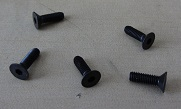
\includegraphics[width=80px]{hw/M3X10FC.jpg}\\
Hex Socket Cap Screw M3 x 0.5mm x 10mm & 367-B04-1P	& 5 & \\
Hex Socket Cap Screw M2 x 0.4mm x 6mm	& 366-663 & 4 & \\
\end{tabular}
\caption{Bill of Nuts and Bolts}
\label{table:screws}
\end{table}

\begin{table}[!h]
\begin{tabular}{p{5cm} | c | c | c | c}
part & supplier & part number & quantity & image \\
\hline
Hook up wire 20-22AWG & various, adafruit & adafruit 1311 & various colors & 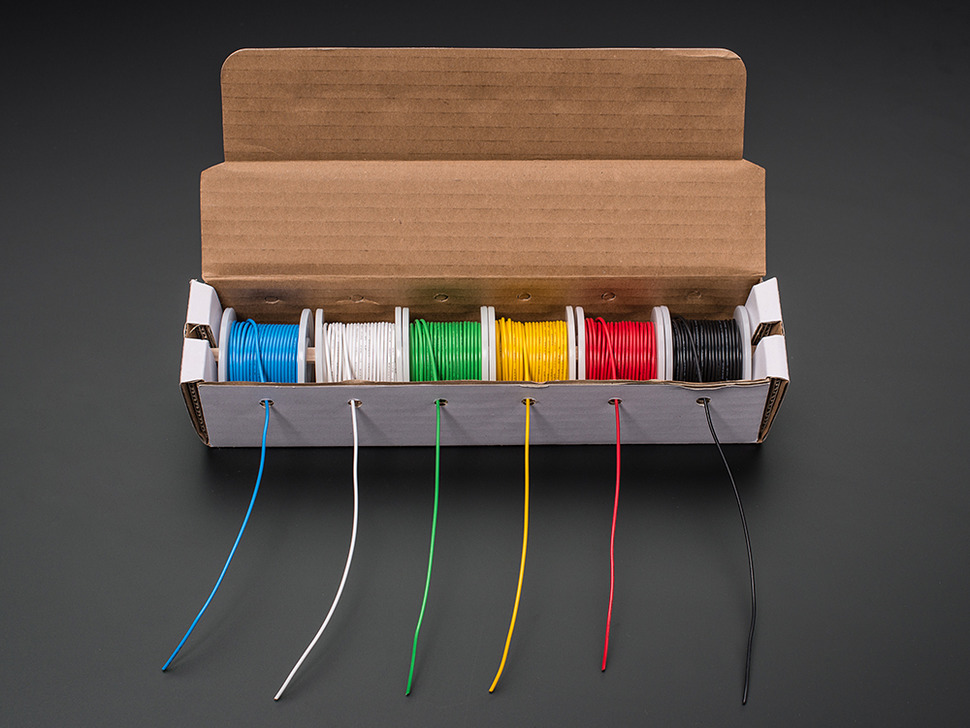
\includegraphics[width=80px]{picture/wires.jpg}\\
Female JST-XH <-> Male Polyquest 3S 10cm (5pcs/bag) & HobbyKing & 101b-103a-3s & 1 & 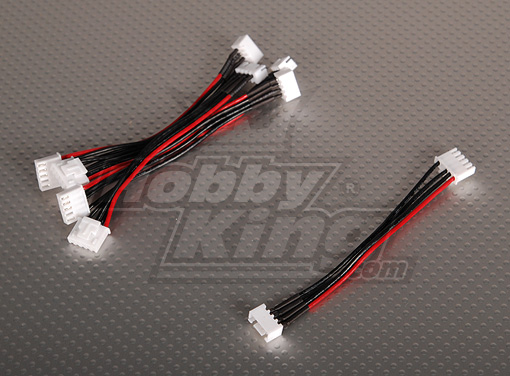
\includegraphics[width=80px]{picture/jstext.jpg}\\
Female JST battery pigtail 12cm length & HobbyKing & AM-9017A & 2 & 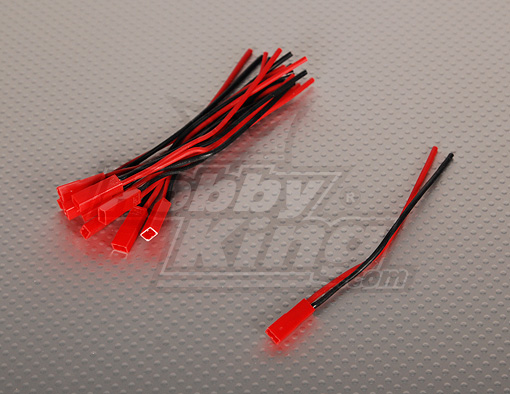
\includegraphics[width=80px]{picture/fjst.jpg}\\
Male JST battery pigtail 10cm length & HobbyKing & AM-9017B & 2 & 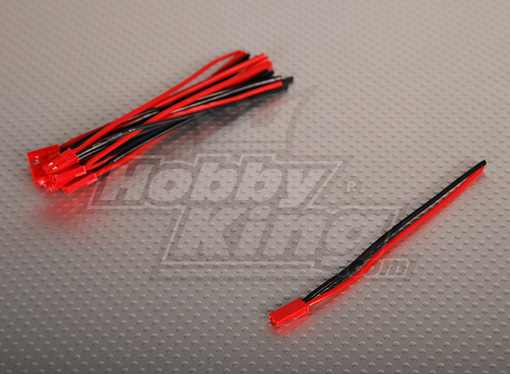
\includegraphics[width=80px]{picture/mjst.jpg}\\
Power Switch SPST & SW627-ND & digikey & 1 & 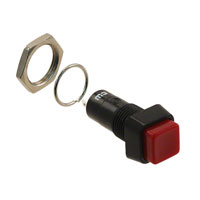
\includegraphics[width=80px]{picture/pwr.jpg}\\
2 pin connector: motor to MCU & Aliexpress, Digikey & & 4 & 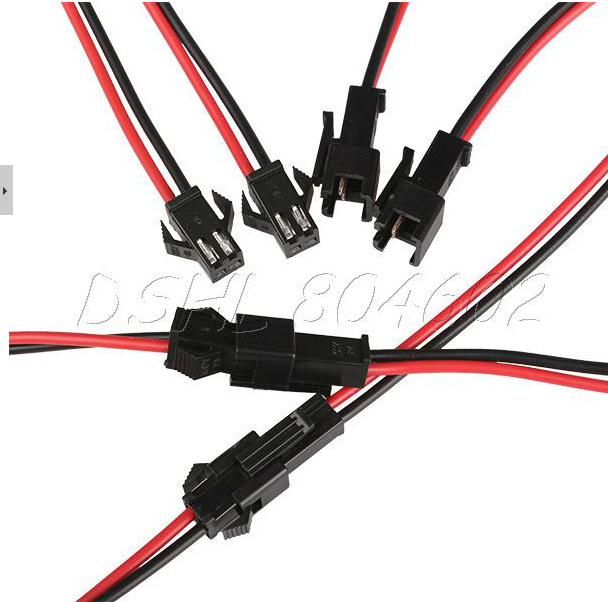
\includegraphics[width=80px]{picture/2pinconn.png}\\

\end{tabular}
\caption{Bill of Wires and Connectors}
\label{table:wires}
\end{table}


\section{3D printing}

The Razbot is made up of 8 unique 3D printed parts and a total of 12 3D printed pieces. The table: \ref{table:3Dprintparts} lists each part which is made with a 3D printer. The Razbot has been previously constructed with the printers listed and tested in Table: \ref{table:3Dprinters}. Note that hex cap screws on this platform thread directly into 3D printed plastic. Holes have been sized appropriately to allow clearance for screws and appropriate diameters for threading. Appropriate hole sizing may vary printer to printer and should be checked on initial prints. Repeated screwing and unscrewing or forcing taps or screws may result in damage to 3D printed threaded holes.  

Some parts will require support material. All parts have been found to function well when printed at 20\% infill. 3D printing settings and parameter decisions will ultimately be left to the operator. 

\begin{table}
\begin{tabular}{p{5cm} | c | c | c}
part & quantity & image & support material required\\
\hline
Side Left V01 & 1 & 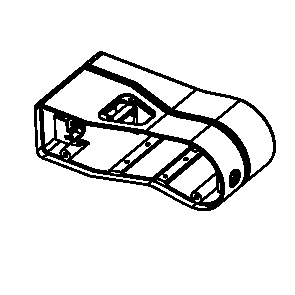
\includegraphics[width=70px]{diagram/Side_Left_V01.pdf} & yes\\
Side Right V01 & 1 & 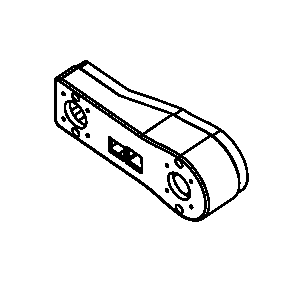
\includegraphics[width=70px]{diagram/Side_Right_V01.pdf} & not required\\
FR motor holder & 1 & 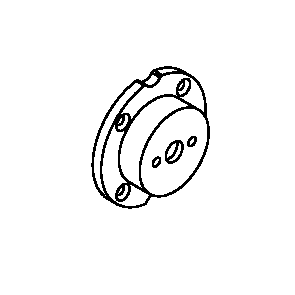
\includegraphics[width=70px]{diagram/FR_motor_holder.pdf} & yes\\
RR motor holder & 1 & 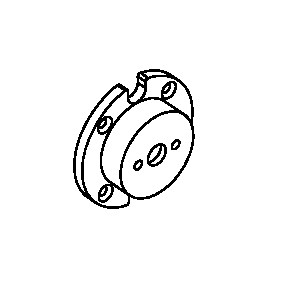
\includegraphics[width=70px]{diagram/RR_motor_holder.pdf} & yes\\
L motor holder & 2 & 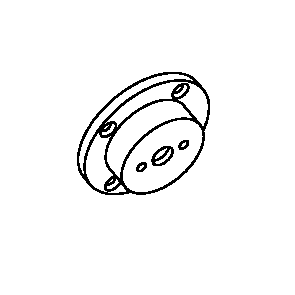
\includegraphics[width=70px]{diagram/L_motor_holder.pdf} & yes\\
PiTrayB & 1 & 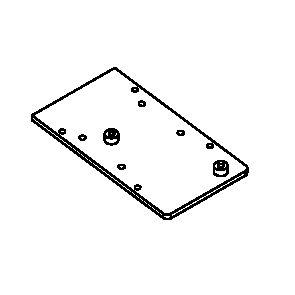
\includegraphics[width=70px]{diagram/PiTrayB.pdf} & not required\\
Top Plate & 1 & 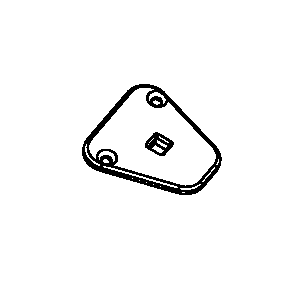
\includegraphics[width=70px]{diagram/Top_Plate.pdf} & not required\\
Wheel & 4 & 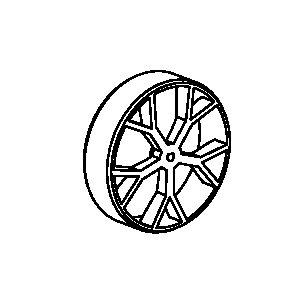
\includegraphics[width=70px]{diagram/Wheel.pdf} & not required
\end{tabular}
\caption{Bill of 3D printed components}
\label{table:3Dprintparts}
\end{table}

\begin{table}
\begin{tabular}{c | c | c | c}
printer & build volume & image& result quality\\
\hline
Makerbot Replicator 2 & 28.5 L X 15.3 W X 15.5 H cm & 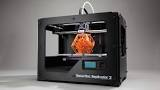
\includegraphics[width=70px]{picture/makerbotrep2.jpg} & excellent $\dfrac{10}{10}$\\
Tinkerines Ditto+ & 21.0 L X 18.5 W X 23.0 H cm  & 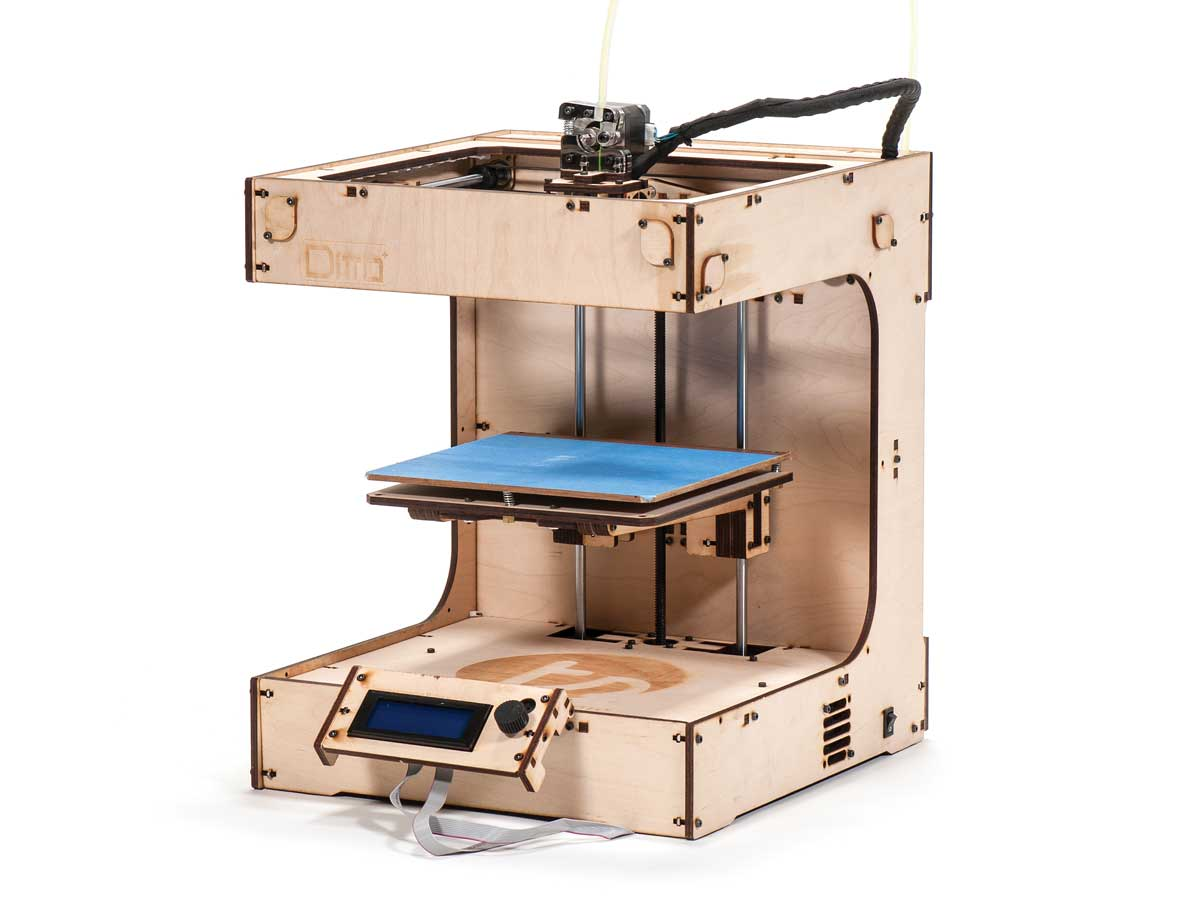
\includegraphics[width=70px]{picture/ditto.jpg} & very good $\dfrac{9}{10}$\\
 
\end{tabular}
\caption{3D printers used}
\label{table:3Dprinters}
\end{table}




\chapter{Assembly}

The rover is easy enough to assemble but it isn't perfect, yet. Many components and wires are packed tightly into a small space. Screws may be difficult to access with hex keys. Once the vehicle has been assembled and is running properly, minimal disassembly and maintenance will be required. Once all the 3D printed components are available with support material removed assembly can begin.\\

\section{Razbot MCU board}

The Razbot MCU board is easy to make with the proper tools and soldering skills. Some of the components are quite small so proper tools and a good deal of patience is important.
\begin{figure}
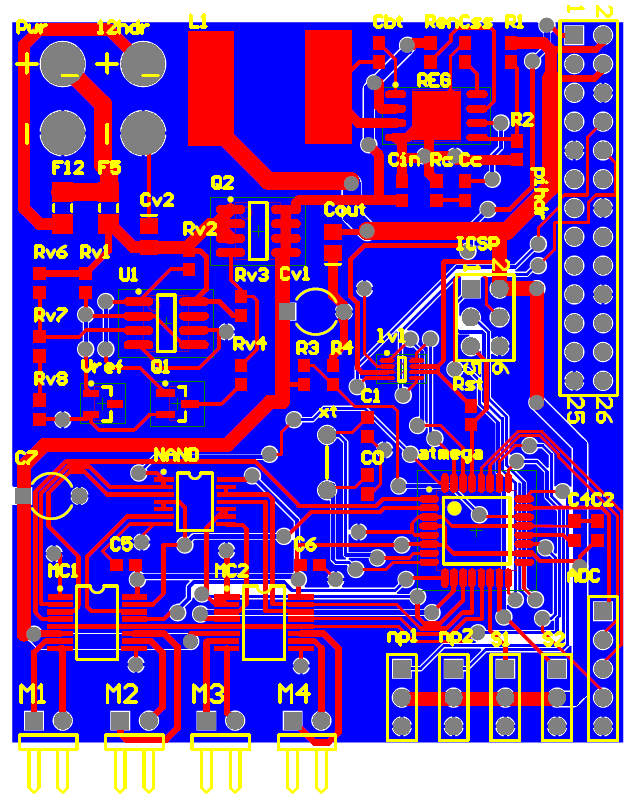
\includegraphics[width=400px]{picture/mcu.png}
\caption{MCU board layout}
\end{figure}
\begin{figure}
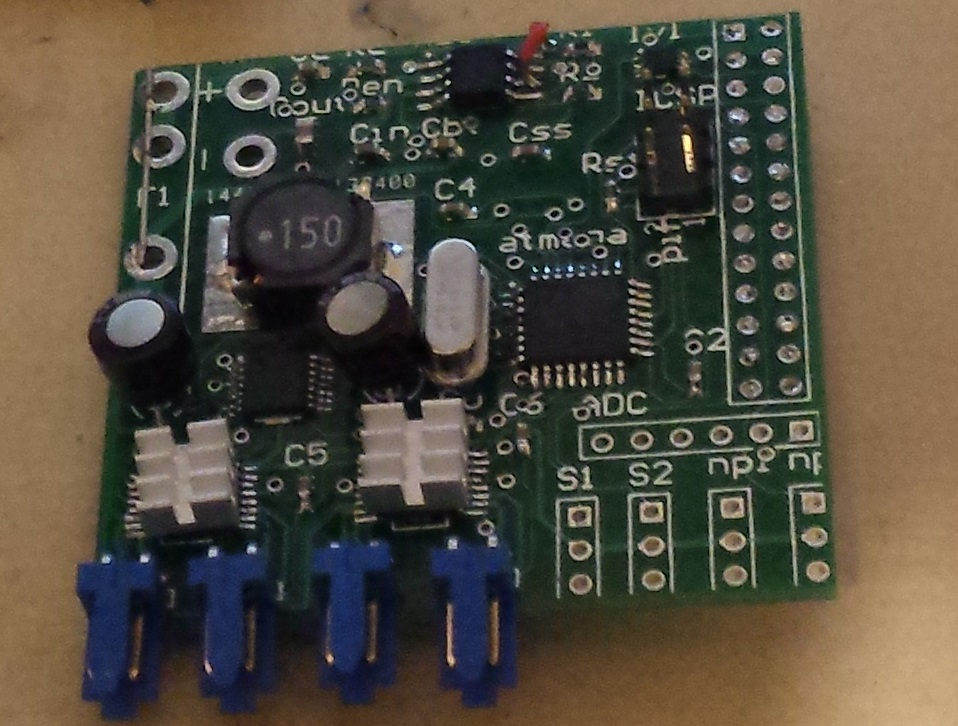
\includegraphics[width=400px]{picture/piboard.jpg}
\caption{A prototype version of the Razbot PCB}
\label{figure:pcbv1}
\end{figure}



\begin{enumerate}
\item The unpopulated PCB board can be ordered from a low cost PCB manufacturer such as \href{http://www.seeedstudio.com/}{SeeedStudio} using the exported PCB design files or Gerber files in the electronics folder. The exported files are zipped in razbot{\_}pcb{\_}output.rar.
\item The electronics components can be ordered from a supplier such as \href{http://www.digikey.com/}{Digikey} or \href{http://www.Newark.com/}{Newark}. The component part numbers and quantities can be found in the excel document razbot BOM.xlsx in the electronics folder.
\item Once the boards and components arrive, the components can be soldered on to the PCB using a fine tipped, temperature controlled soldering iron. Tweezers will greatly assist in placing components. Proper use of flux will ensure easy soldering without jumping component pins. Solder the components on to the board following the designators on the board (also found in the razbot schematics pdf in the electronics folder) and the designator table in the Bill of Materials for the electronics components.\\
The power regulator chip RT8250 has a ground pad on the bottom surface of the chip which requires an electrical connection with the board. A hot air station can be used to reflow solder on the PCB and attach the chip. Conductive paste may also be an easier solution.
\item Use the AVRISP-mkii programmer with the Arduino IDE to load the Arduino bootloader on to the ATmega328P on the MCU board by connecting to the ICSP header on the board. This will set the proper fuse bits on the ATmega328P for use with Arduino code.
\item Use the programmer again to load on the razbot arduino V02 code located in the razbot Software MCU folder. The ros lib library must be played in your Arduino IDE's libraries folder to compile the code. 
\end{enumerate}

\begin{figure}
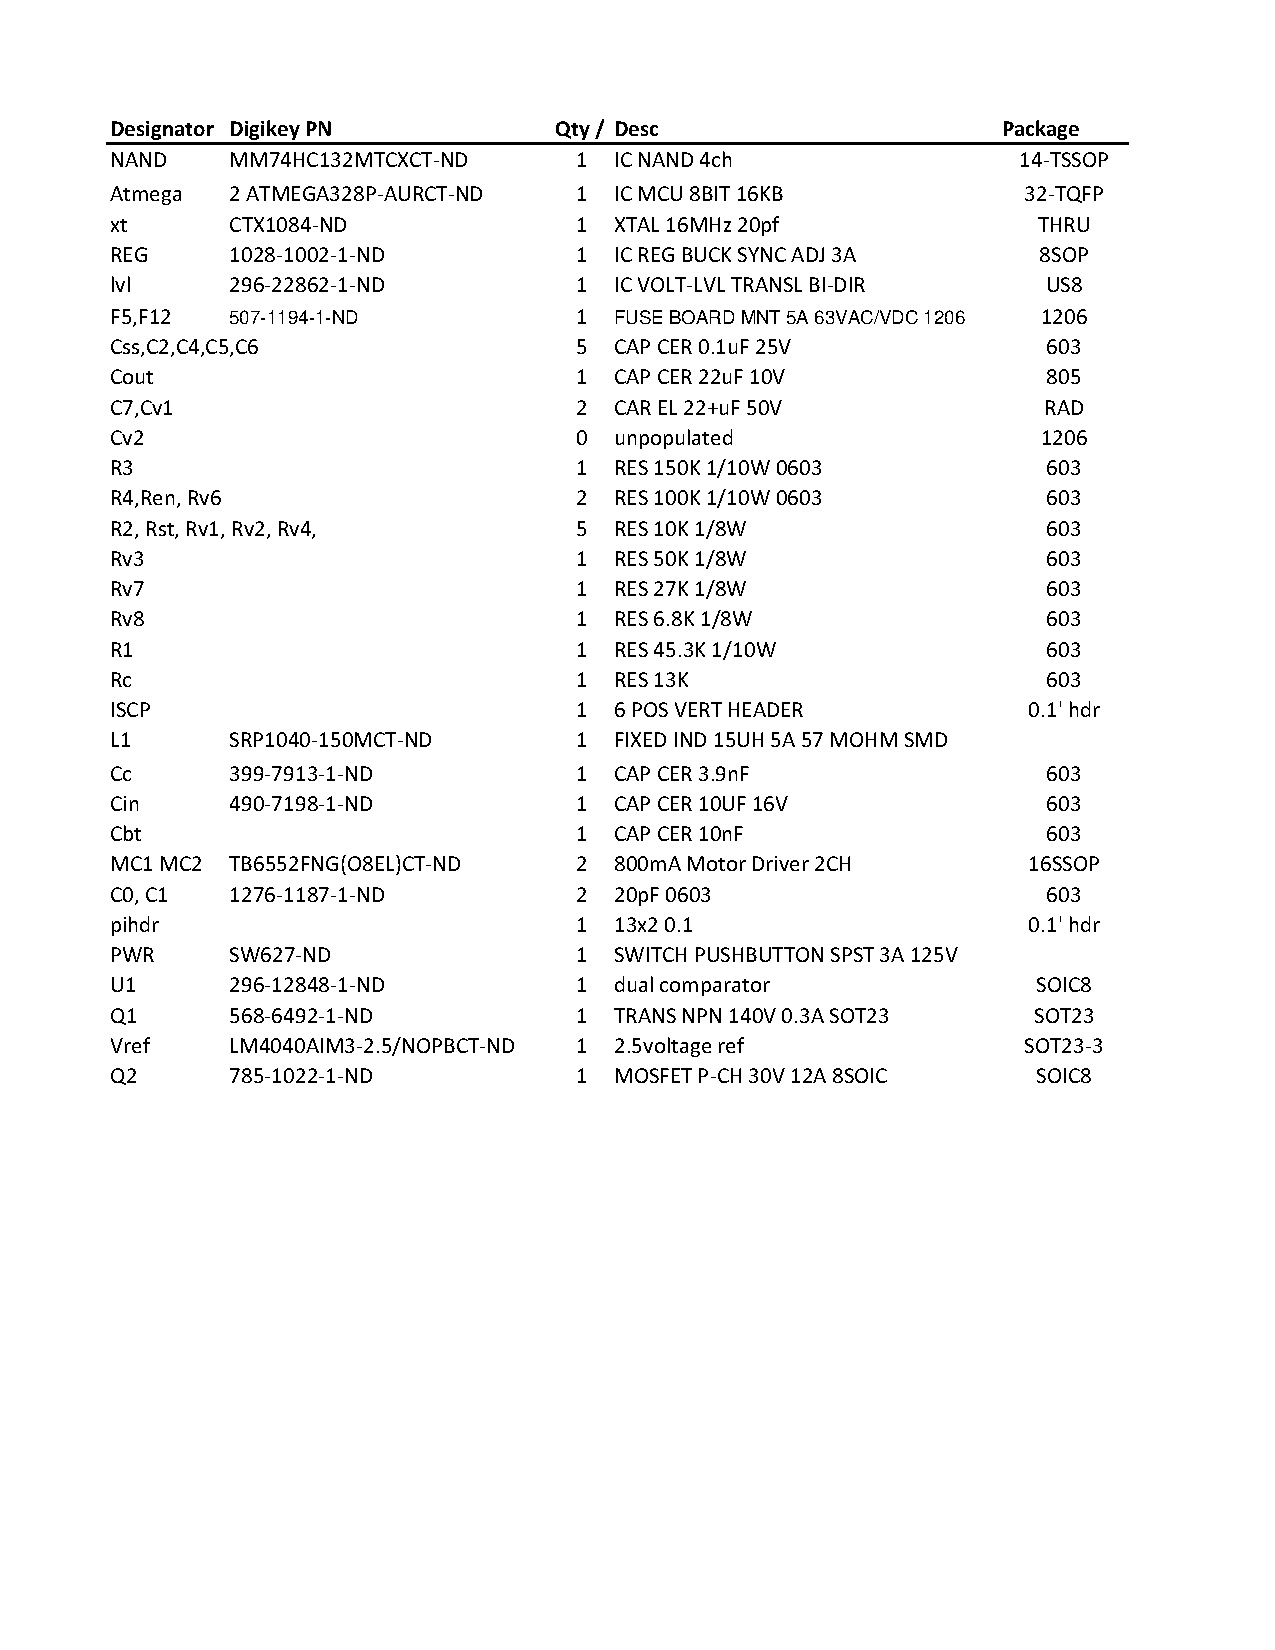
\includegraphics[width=40pc]{hw/razbot_BOM.pdf}
\caption{MCU electronics board bill of materials}
\end{figure}

\subsection{MCU Board Alternatives}

Ordering and assembling your own PCB may seem like a daunting task. Razbot was originally developed using off the shelf components connected to a Raspberry Pi. This may be appealing to users not wanting to create their own PCB so some guidelines are presented here. Note that the increase in wiring can result in larger potential for error and possibly more work than building the PCB in the first place.

Razbot was initially build with an Arduino Micro mounted to the GPIO pins on the Raspberry Pi connected to the serial port. This could have also been connected over USB. It was used to control an L298 2 channel motor driver as well as other servos. A Turnigy 5V 5A switching regulator was used to supply 5V to the robot from the 11.1V Lithium battery. Users may be able to do away with the Arduino Micro and simply drive the L298 motor controller with the Raspberry Pi GPIO. 

Squeezing components into the small Razbot chassis may prove difficult. The Razbot has 4 motors, thus the 2 motors on each side of the vehicle must be wired in parallel removing potential for future omnidirectional upgrades.

The components for the MCU board alternative solution are listed in \ref{table:altparts}.

\begin{table}[!h]
\begin{tabular}{p{5cm} | c | c | c }
part  & supplier  & cost & image \\
\hline
Arduino Micro & Adafruit &  \$22 & \\
L298 2 ch motor controller & Aliexpress, Ebay, Seeedstudio &  \$4-20 & \\
Turnigy 5V 5A Switching Regulator & HobbyKing &  \$5 & \\

\end{tabular}s
\caption{Parts for MCU alternative robot}
\label{table:altparts}
\end{table}


\section{Electronics Assembly and Test}

\begin{enumerate}

\item Download the latest Razbot SD card image from \href{https://drive.google.com/file/d/0B4yfrdhk2e0OVlA1alJoRXBPeXM/view?usp=sharing}{SD card image on Google Drive}. Extract it with Winrar and use a program such as Win32diskimager to mount it on to an 8GB SD card. Later when the image is booted, raspi-config can be used to expand the file system to fill the full 8GB of storage.\\
\textbf{Raspberry Pi B only!}\\
The current SD card image does not support the Raspberry Pi 2. It can be easily updated to run on the RPi2 by updating the firmware following instructions on the internet such as (\textbf{INSERT LINK}). The next image update will be RPi 2 compatible.

\item Plug the Raspberry Pi Camera and Wifi dongle into the Pi and insert the SD card for now. Connect the unit to an Ethernet port on your router. Use conventional wall power to power the unit.
	\begin{enumerate}
	\item  Using your router's user interface, locate the IP address of the Raspberry Pi. The initial hostname will appear as <color>pibot. This can be changed with raspi-config at a later time.
	\item SSH into the Raspberry Pi using the IP address from step 2.1. In windows this can be done with a free program such as \href{http://www.chiark.greenend.org.uk/~sgtatham/putty/download.html}{Putty}. Username and 			password as usual:\\
	username: pi\\
	password: raspberry\\
	\item Verify that ROS is running (robot upstart is used to start ROS and required nodes at boot up).\\
	\begin{verbatim}
		$rostopic list
	\end{verbatim}
	\item Verify the mjpg-streamer software has started and is streaming video from the camera. Point a web-browser to: Your bot's IP address:8080
	Configure the Wifi on the Pi to automatically connect to your network using wicd-curses.
	\begin{verbatim}
		$sudo wicd-curses
	\end{verbatim}
	\end{enumerate}

\item Attach the wire ends of a male JST pigtail connector to the Lithium Polymer battery.\\
	\begin{enumerate}
	\item Using a hobby knife, remove a small amount of shrink wrap from the battery ground (black) wire connection to the yellow XT-60 connector.
	\item Solder on the ground (black) wire to the JST connector
	\item repeat this process with the positive (red) connection on the yellow XT-60 connector
	\item Solder on the positive (red) lead from the JST connector\\
	\end{enumerate}
	\begin{center}\textbf{WARNING}\end{center}
	Take care not to short the battery terminals together while making this modification. Do not let the knife short the terminals while cutting!\\
	\begin{center}\textbf{WARNING}\end{center}
	Take care to check the polarity of the connection, red to red, black to black.
	\item Mount the MCU electronics board on top of the Raspberry-Pi. Ensure the GPIO connectors line up with the female header on the MCU board.
	\item Wire connectors to the electric motors
	\begin{enumerate}
		\item Cut 10cm lengths of two different colors of 20-22awg wire for each of the motors (4x color 1, 4x color 2)
		\item Solder one end of each wire to the motor terminals, ensure consistency of polarity. Check for the red dot on the motor by the terminal to find the positive connection.
		\item Build the 2pin blue connector (PART NUMBERS) on the other ends of the wires for each motor. Again, ensure consistency of polarity. Place positive on the right and side of the connector (connector slot faces upwards)	
	\end{enumerate}
	\item Attach the motors to the MCU board according to the diagram in FIGURE WHAT?
	\item Power up the system by connecting the Battery JST connector to the JST connector on the MCU board. The LED will illuminate in blue. The Pi should power on and boot as usual. 
	\item Verify the system has booted normally, SSH into the Pi and verify ROS and the camera have started.
	\item Verify the motors are operational by manually publishing their control ROStopic
	\begin{enumerate}
	
	\item Set all motors to full forward speed
	\begin{verbatim}
	$ rostopic pub /piBot_motors std_msgs/ColorRGBA 255 255 255 255
	\end{verbatim}
	\item Set all motors to full reverse speed
	\begin{verbatim}
	$ rostopic pub /piBot_motors std_msgs/ColorRGBA 0 0 0 0
	\end{verbatim}
	\item Set all motors to zero speed
	\begin{verbatim}
	$ rostopic pub /piBot_motors std_msgs/ColorRGBA 127 127 127 127
	\end{verbatim}
	Consider the location of each motor on the vehicle when noting the direction of travel of each
 motor.
 	\end{enumerate}
 	\item Verify the LED is responsive by publishing color topics. Set the light to red+green
 	\begin{verbatim}
 	$ rostopic pub /piBot_led std_msgs/ColorRGBA 180 120 0 0
 	\end{verbatim}
 	\item Verify the battery voltage is being monitored properly.
 	\begin{verbatim}
 	$ rostopic echo /piBot_bat
 	\end{verbatim}
\end{enumerate}
The electronics bring-up is complete

\begin{figure}
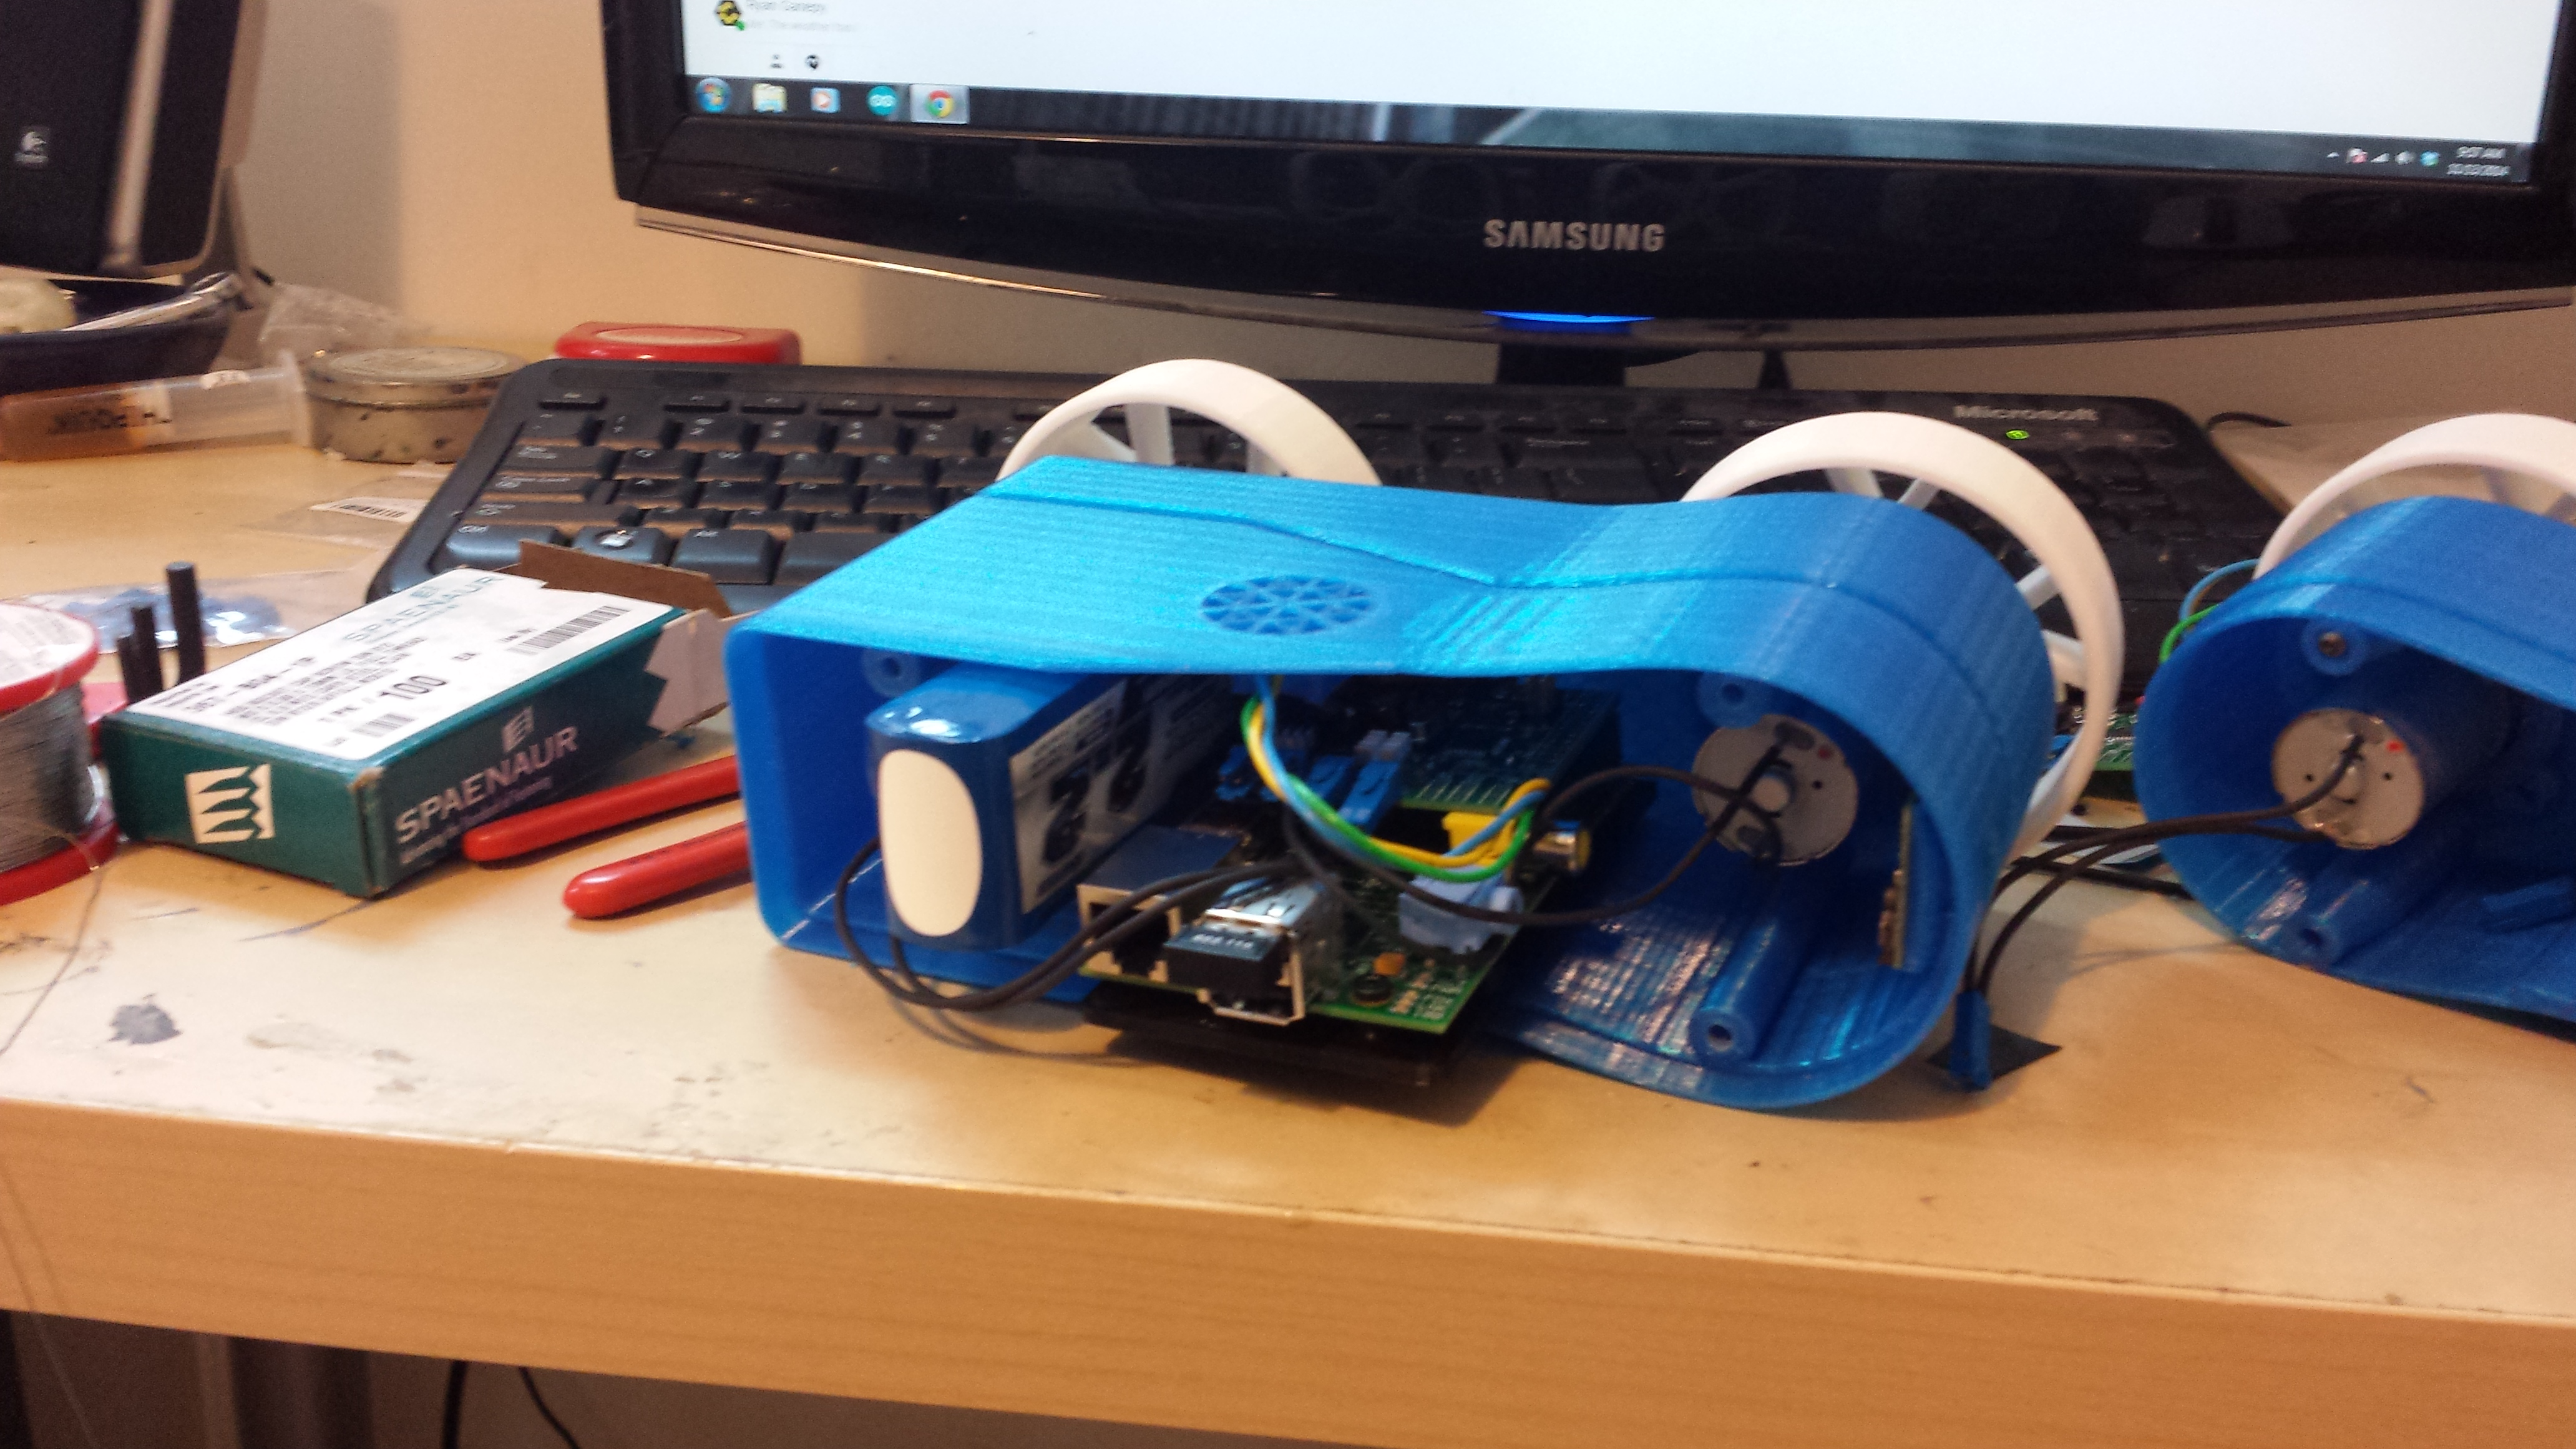
\includegraphics[width=400px]{picture/side.jpg}
\caption{Electronics assembled, mounted in chassis}
\end{figure}

\section{Mechanical Assembly}

\begin{enumerate}
\item Attach the Pi-Tray to the left side of the chassis (PiTrayB to Side Left V01) using 2-4 Hex Socket Low Head Cap Screw M3 x 0.5mm x 5mm screws.\\
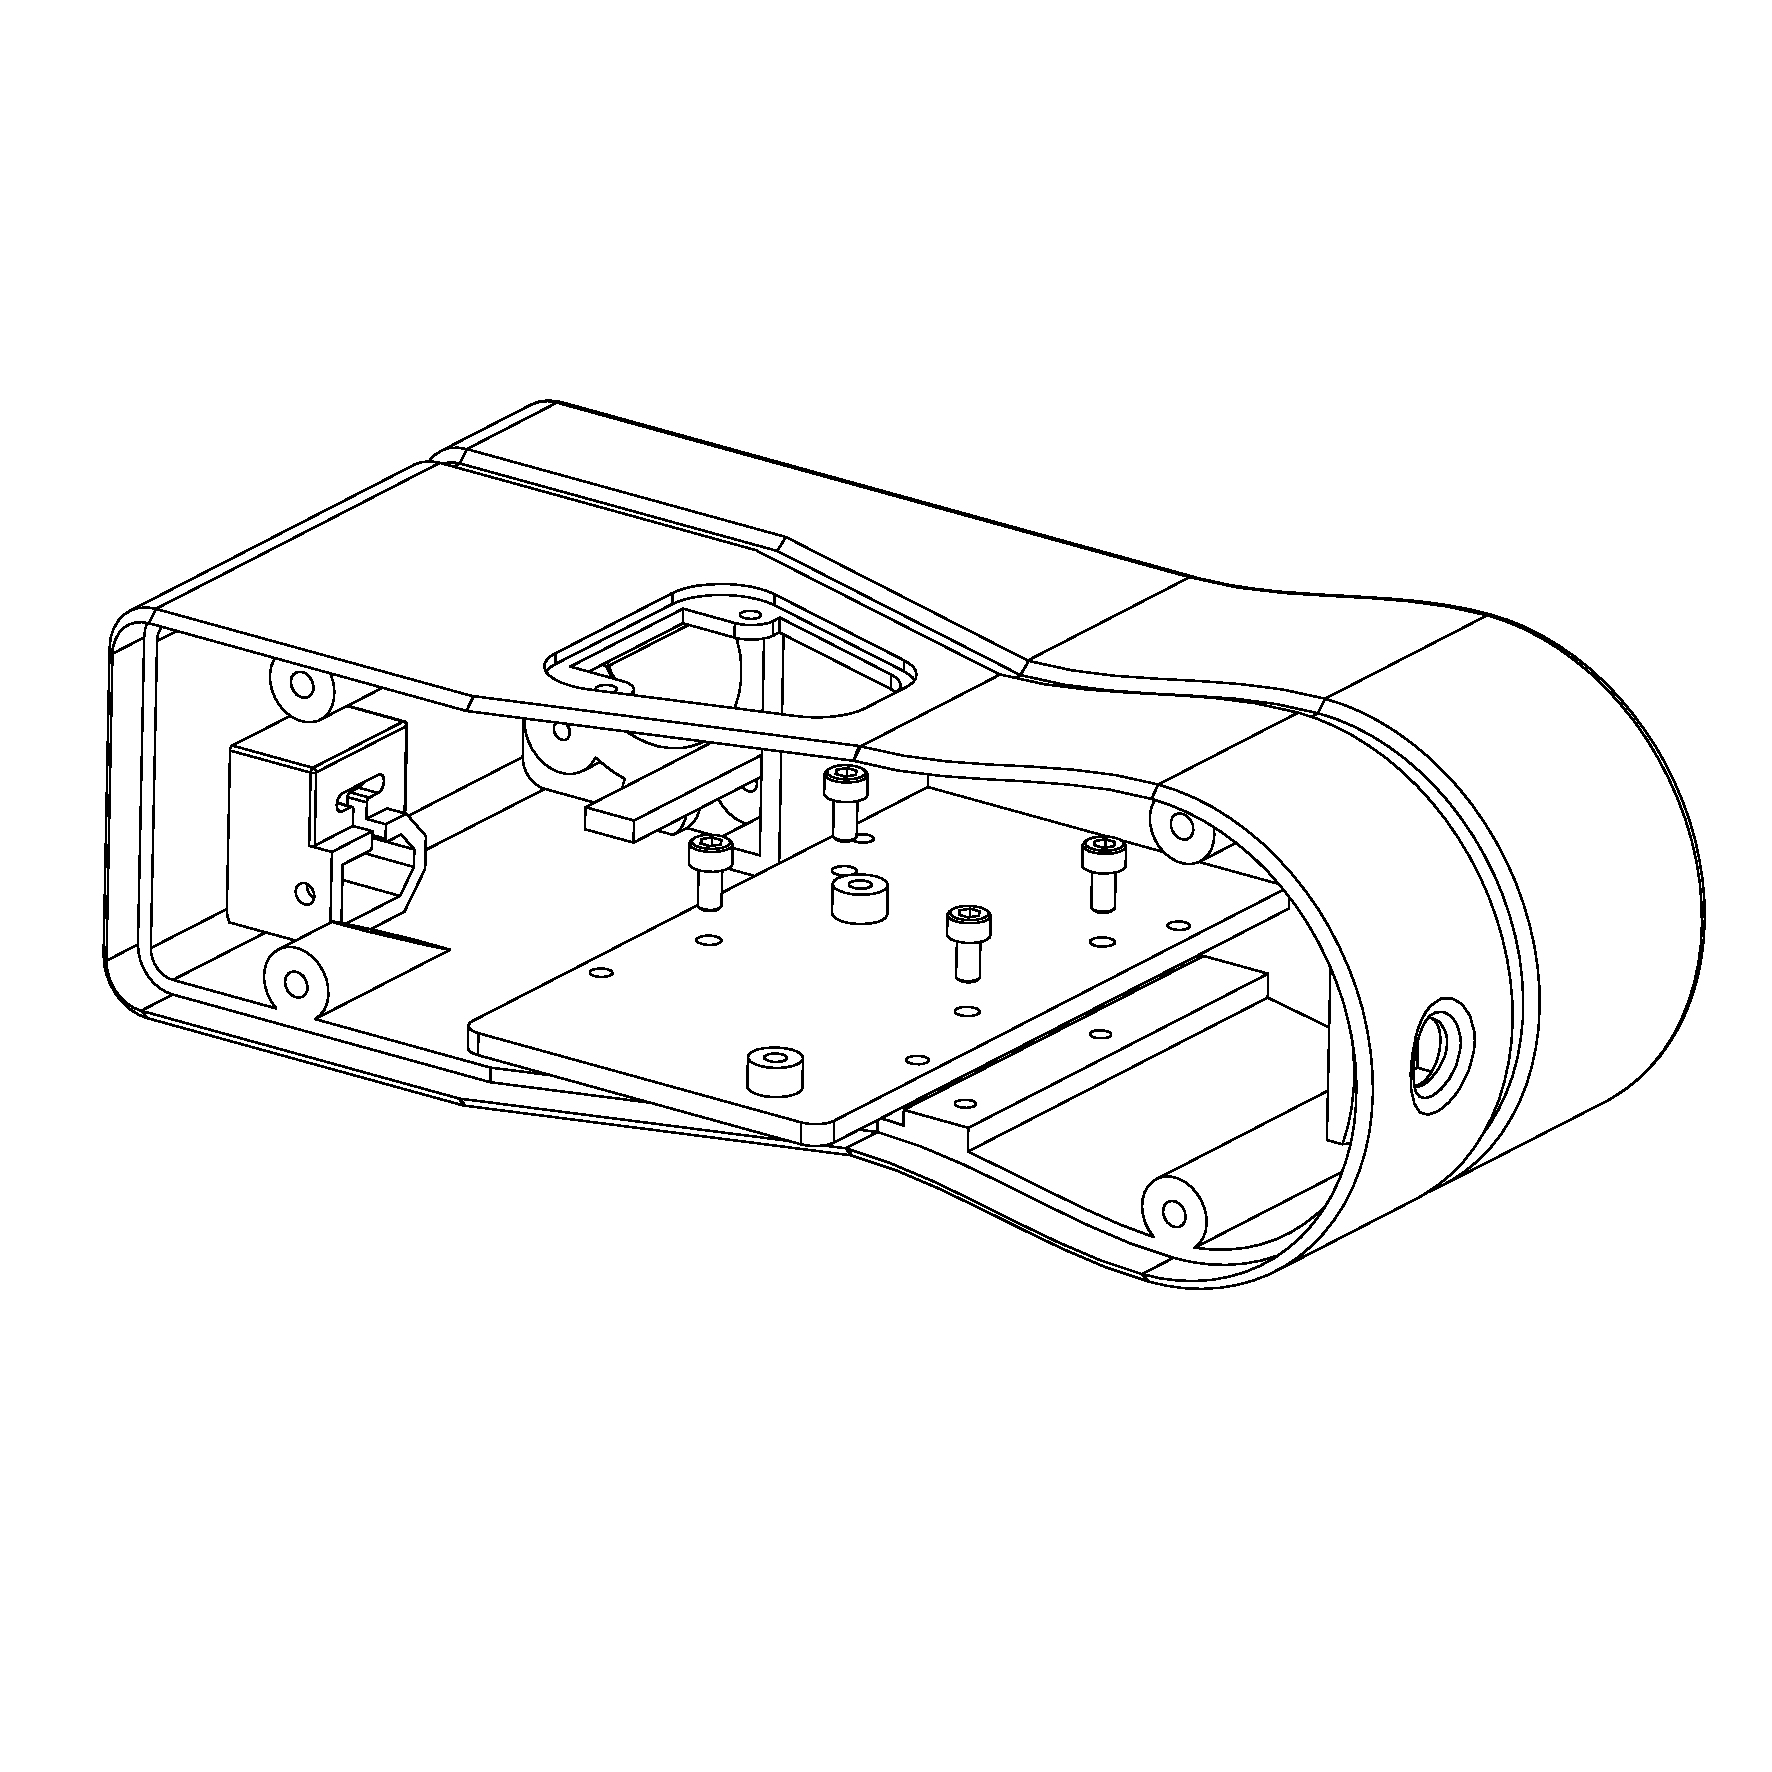
\includegraphics[width=400px]{assem/step1.PDF}
\item Mount the Pi-Camera to the inside of Side Left V01 using M2 Hex Cap Screws. Leave the ribbon cable attached to the camera board but not to the Pi during this process.
\item Install the Pi on the Pi mounting tray using M3 x 0.5 x 6mm Low Head Hex Cap screws
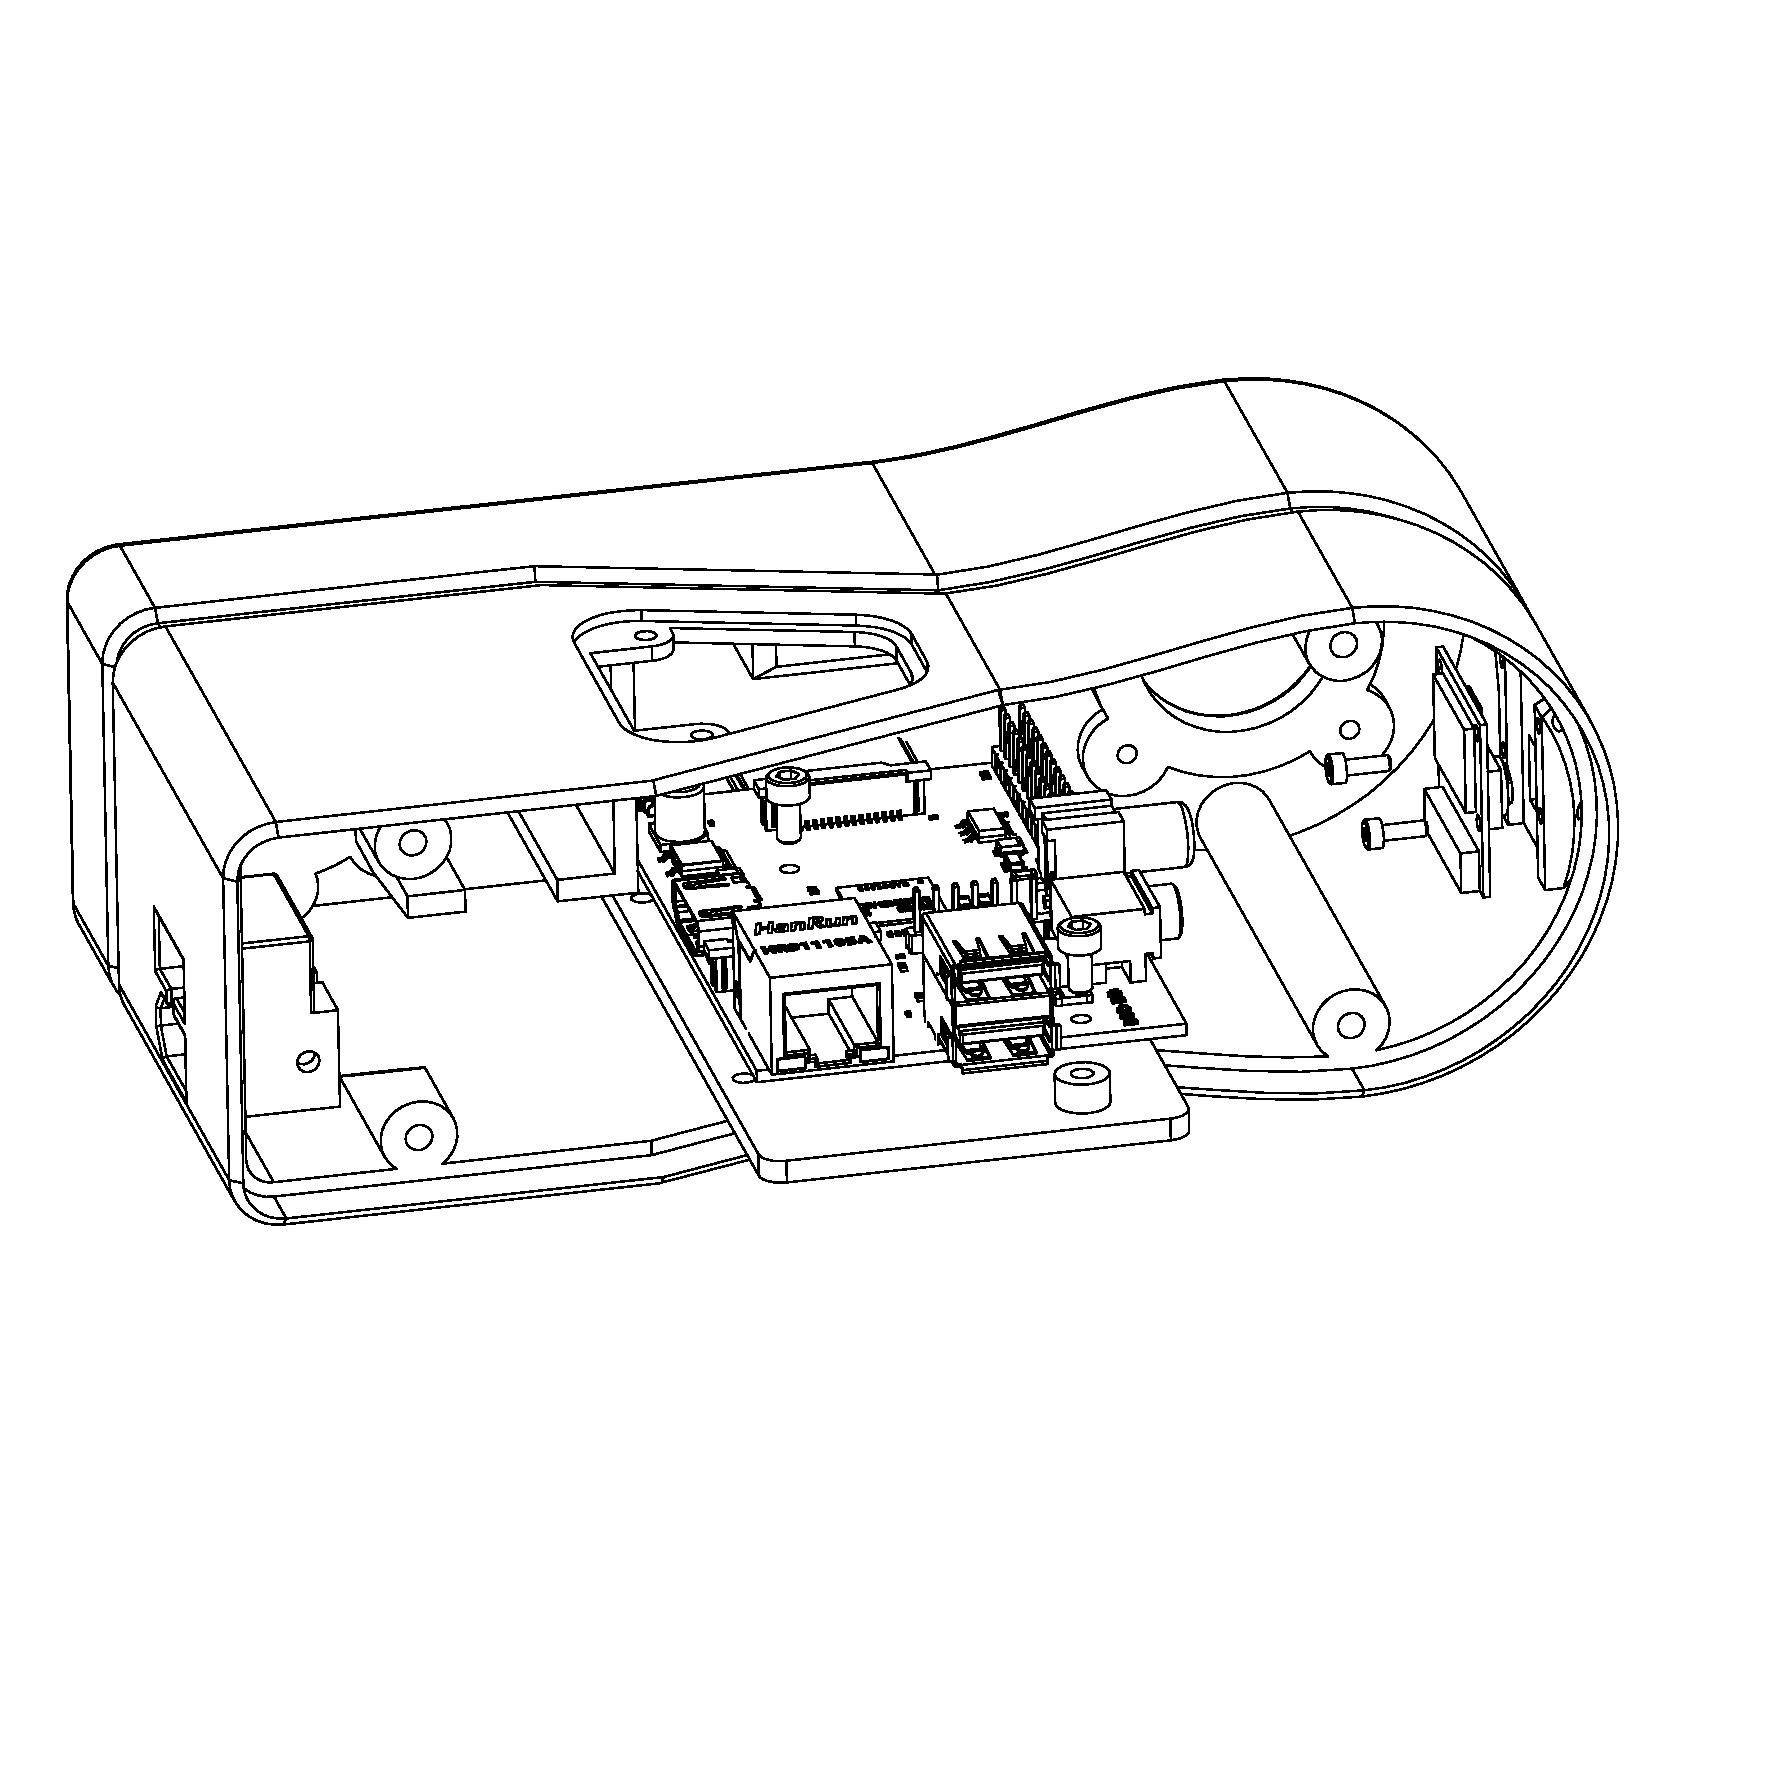
\includegraphics[width=400px]{assem/step2.PDF}[h]
\item  Attach the JST connectors to the power switch as shown in Figure <MAKE A FIGURE>. Positive power should run though the switch.
\item Install the switch into the slot in Side Left V01
\item Install the battery into Side Left V01. Before fully inserting the battery, run the balancing plug out the rear connection socket of the robot. This can be difficult, take care not to damage the wires. Next run the XT 60 out the corresponding rear connection socket. Run the JST back in the robot towards the Pi mounting tray. Fully insert the battery.
\begin{enumerate}
	\item Lock the XT-60 connector in place with the M3 x 0.5 x 6mm Low Head Hex Cap set-screw
\end{enumerate}
\item Connect the battery JST to the switch.
\item Connect the switched JST power to the MCU board. Test the functionality by turning it on. Ensure the electronics are not in contact with metal surface or other potential shorts during testing. Remove the MCU Board. 
\item Connect the Pi camera ribbon cable to the Pi.
\item Push the LED and wiring through the hole in Side Left V01. Attach the LED to the Top Plate using M2 screws if possible or just hot glue. Screw the Top plate down to Side Left V01 using M3 x 0.5 x 10mm Flat Head Hex Cap screws.\\
\item Install the motors in each of the motor holders using M3 x 0.5 x 6mm Low Head Hex Cap screws.
\item Push the wheels on to the motor shafts. This may require a tap from a hammer. Use M3 x 0.5 x 10mm set screws in the wheels if required.\\
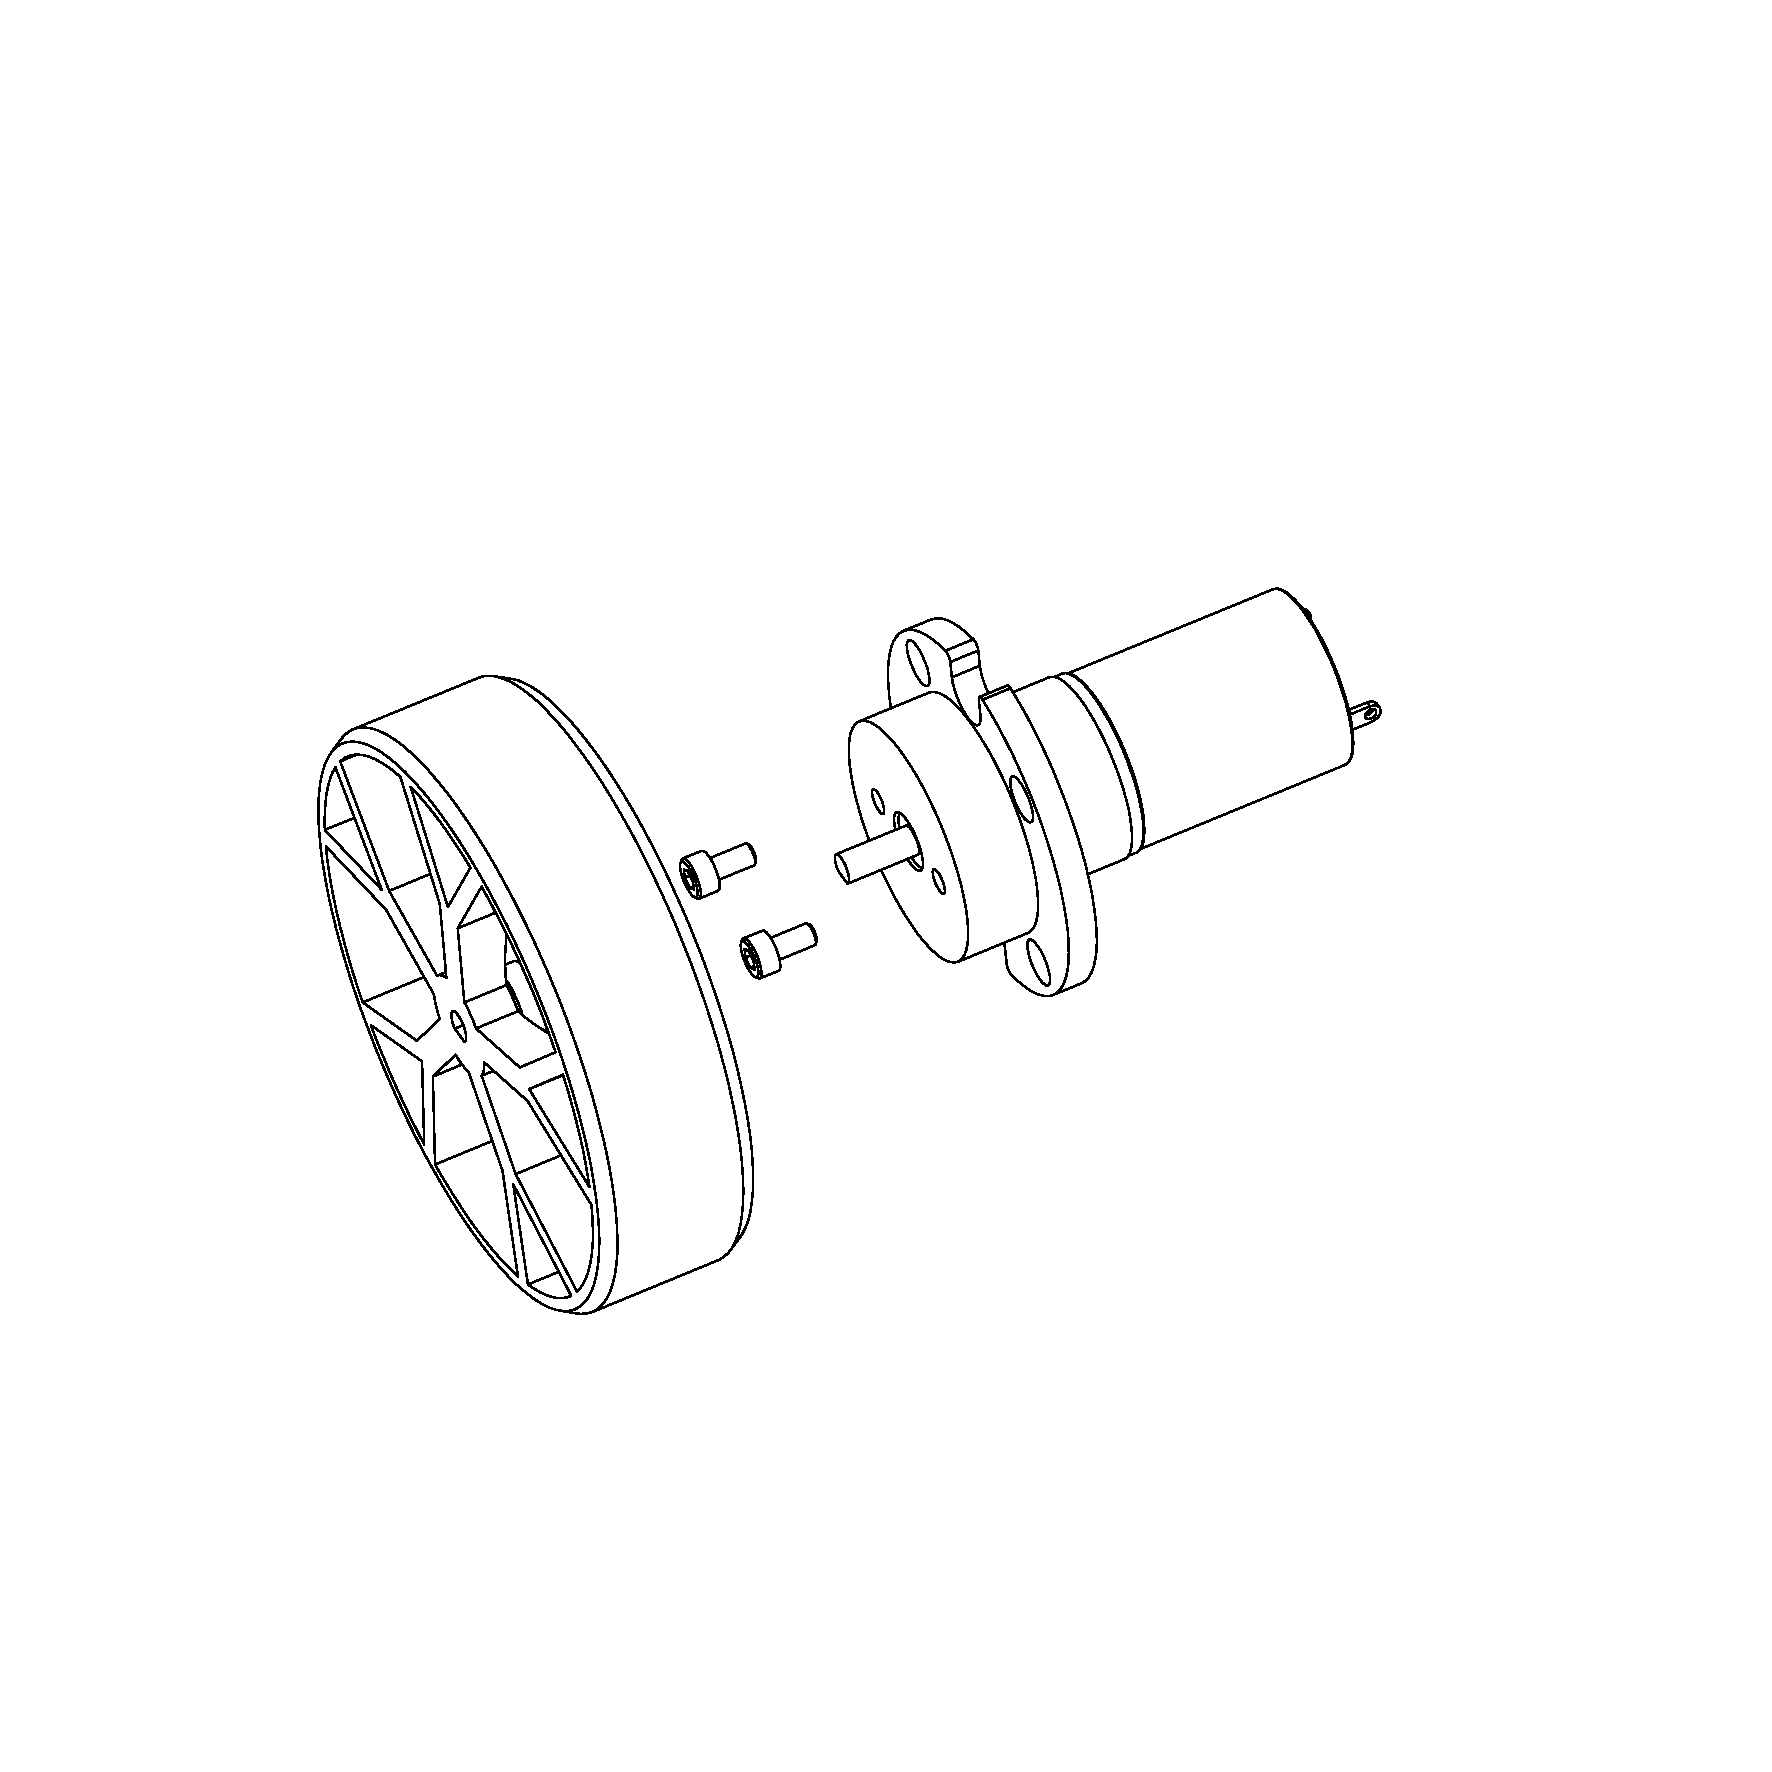
\includegraphics[width=400px]{assem/step3.PDF}[h]
\item Install the motor holder assemblies into the vehicle chassis sides (Side Left V01, Side Right V01) using the M3 x 0.5 x 10mm flat head cap screws.\\
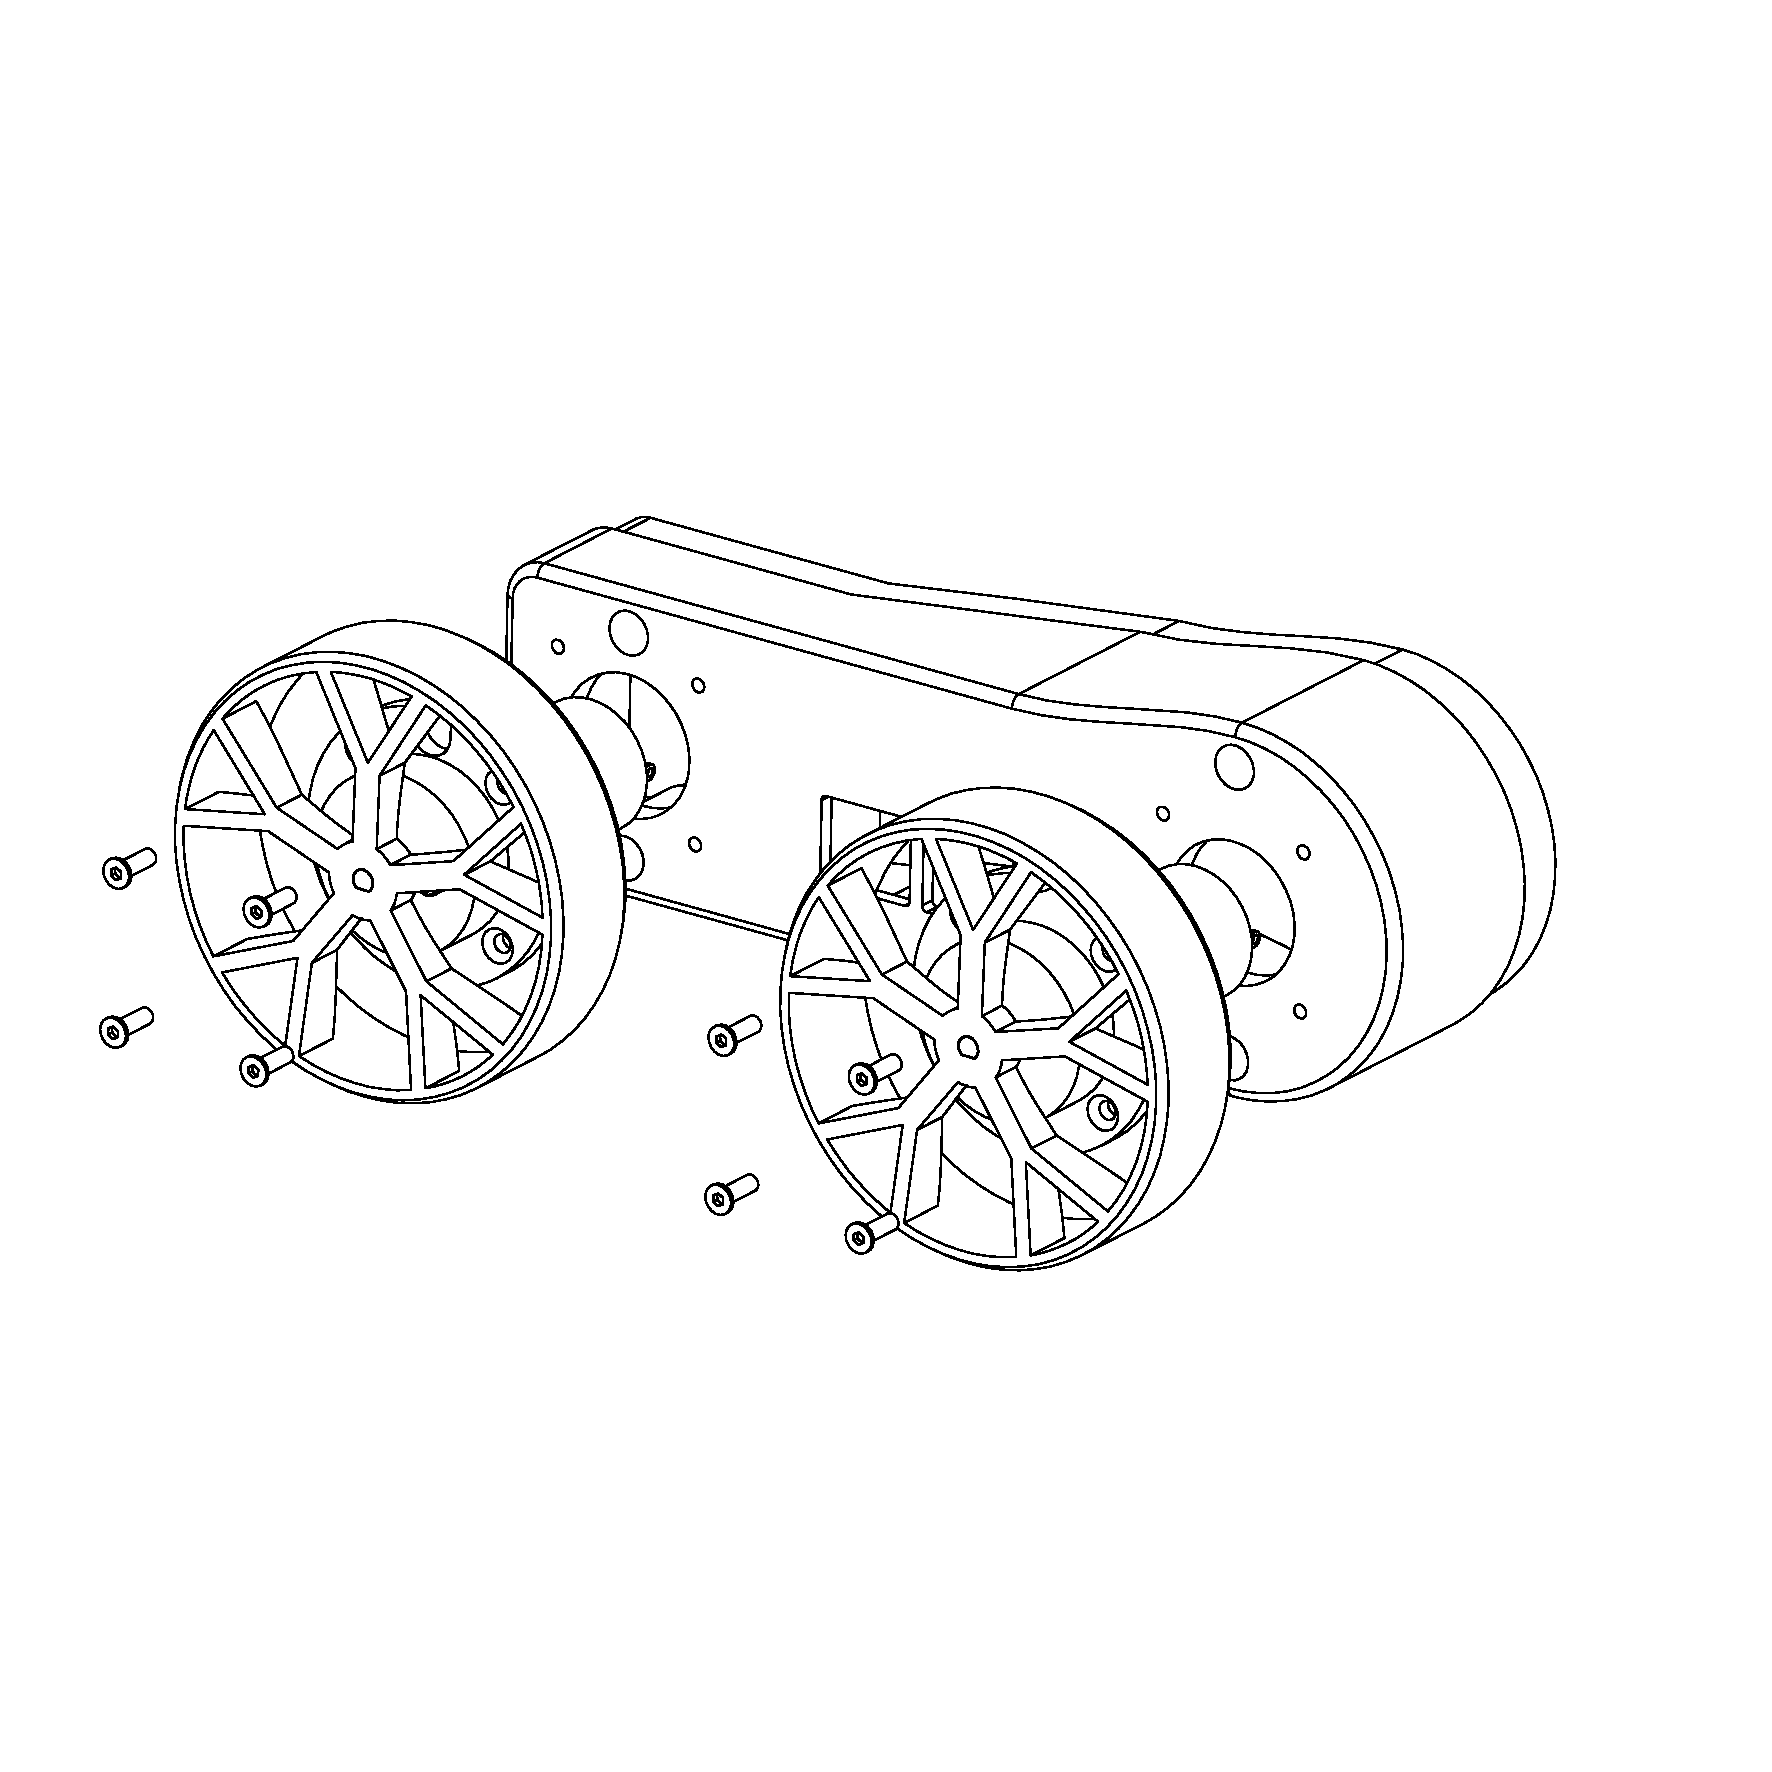
\includegraphics[width=400px]{assem/step4.PDF}[h]
\item Connect the motor wires to the MCU board in proper order shown in Figure XXX. You may wish to verify proper operation of the electronics one more time at this points.\\
\item Push the two sides of the vehicle together while taking care not to tangle or stress wiring. This may take patience. 
\item Use four M4 x 0.7 x 25mm bolts to attach the chassis sides together.

\end{enumerate}

Mechanical assembly is complete.

\chapter{Operation}

The Razbot is easy to use! Simply turn it on and begin enjoying your ROS-robot experience.
Razbot uses the ROS robot upstart package to launch its ROS nodes.

\begin{enumerate}
\item Press the Red power button on the left side of robot. The status LED will illuminate Blue
\item Give the robot some time to boot up. The red camera light will come on and shine through the 3D printed chassis at the front when launch is complete. Joystick control will also be available if a USB gamepad joystick is plugged in.
\item Locate your robot's IP address with your router. Log into your router, typically located at 192.168.1.1 and find the IP address assigned to the razbot hostname. In some case you will be able to use the hostname (razbot) in place of the IP address
\item Navigate to the server hosted by mjpg-streamer at  (robot-IP-address):8080 or (robot-hostname):8080.
\item To control the robot using a browser and view the video feed, navigate to (robot-IP-address):8080/ROScontrol.html. (Currently Unfinished but works)
\end{enumerate}

\section{ROS Operation}

The Razbot will start some of it's own software when the Raspberry Pi boots up. This will allow it to connect to a USB joystick and drive the rover as well as view the camera and accept commands from a web browser.

To view the ROS nodes which are run on start-up type:
\begin{verbatim}
$rosnode list
\end{verbatim}

The following nodes should be enumerated

\begin{itemize}
\item pibot - subscribes to the joy topic and publishes piBot motors, piBot light
\item joy - publishes the joy topic using a Linux Joystick device
\item rosbridge{\_}server - opens a websocket to receive topics from ROSlibjs
\item rosserial{\_}python - interface with the MCU board to transmit topics
\end{itemize}

A script is also used to start Mjpg Streamer with the Pi Camera\\

To begin working in more depth with the robot and developing your own software, you can SSH into the robot to see what is really going on and run your own code. Use a program such as Putty in Windows to connect to the robot's IP address (determined from your router's DHCP client list). In some cases using the robot's hostname (razbot) will also work. From Linux, simply open a terminal and type:

\begin{verbatim}
ssh pi@<IP address or hostname>
\end{verbatim}

\begin{verbatim}
ssh pi@192.168.1.101
\end{verbatim}

\begin{verbatim}
ssh pi@razbot
\end{verbatim}

The following ROS topics will be visible after start-up by running:
\begin{verbatim}
$rostopic list
\end{verbatim}

\begin{itemize}
\item piBot{\_}motors
\item piBot{\_}light
\item piBot{\_}bat
\item joy
\end{itemize}

To view the data being transmitted in a given topic type:
\begin{verbatim}
$rostopic echo joy
\end{verbatim}
Move the joystick around and watch the data update. Try this for different topics.

\subsection{software disclaimer}
With the electrical and mechanical design now in a somewhat stable state, development work will now focus on updating some of the software on the robot. There may be frequent changes to the razbot packages and the topics and instructions listed above may not always be recent or accurate. Some of the nodes will be reimplemented in a more \textit{standard} fashion of the Robot Operating System. For example: the pibot package will likely be reimplemented using a standard diff-drive controller outputting the cmd vel topic. This will be subsequently used by a razbot base package and a different message type to control the motors.

\section{Simulation and Visualization}

Paul Bovbel has created a URDF (Universal Robot Description File) and a ROS package which allows the Razbot to be simulated in the Gazebo physics simulation environment. Gazebo is a popular tool for roboticist to simulate their platforms, software and sensor arrangements in a virtual environment.

Paul has created tutorials and files which will guide users through setting up the simulation. These are partially available for now (awaiting permission) on \href{https://github.com/Waterfox/razbot_tutorials}{Github}.



\chapter{Future Work}

There remains much to do and much to work on with the Razbot, the following are a few ideas.

\section{software}
\begin{enumerate}
\item update ROS packages to standard format, consistent with gazebo simulation
\item rename ROS topics and packages from pibot to razbot
\item update RPi SD image to be compatible with RPi2
\item Provide a demonstration or control interface with RVIZ
\item Continue development of the Web based camera and control interface. Improve latency
\item update the MCU firmware to accommodate all of the above
\end{enumerate}

\section{electrical hardware}
\begin{enumerate}
\item integrate one or two optical flow sensors to provide odometry to the robot. Update the MCU board to support the sensors. Attempt to do this experimentally on an existing Razbot with and additional Arduino Micro connected over USB.
\item Provide breakouts for additional power and communications on the robot chassis. Break-out the fused 12V power on the robot chassis and make the servo PWM outputs available on the chassis and as a ROStopic for control
\item Add an inertial measurement unit such as the MPU-6000 to the MCU board if cost feasible on the next revision.
\end{enumerate}

\section{mechanical hardware}
\begin{enumerate}
\item Develop or adapt 3D printed Mecanum wheels for the razbot. Implement the appropriate control hardware.
\item Improve assembly ergonomics, access to screws required for assembly, reliability of screw hardware in 3D printed holes
\item Create new industrial design options so users can chose the look of their Razbot
\item Develop better sensor and additional hardware capabilities
\item Modify the wheel design and material to improve \textit{off-road} and carpet capability
\end{enumerate}

\section{general robotics}
\begin{enumerate}
\item Borrow a laser scanner such as an RP-600, SICK TIM 551 or Hokuyo UST 10LX and attempt to run SLAM (Simultaneous Localization and Mapping) as well as autonomy on the robot.
\item Do some form of computer vision or visual SLAM with the RPi camera.
\item offload intensive processing to a server from the RPi.
\end{enumerate}

\section{Final Notes}
If you are attempting to build your own Razbot or are even thinking of building your own system, please drop me a line! Rob.a.Edwards@gmail.com.

Don't hesitate to send any suggestions for improvements, new ideas, questions, requests for support or even complaints. If the documentation is insufficient, let me know or post an issue to the github with where you are having trouble building your bot.

If you do anything cool with your bot, please share! Send pictures, videos, software.

Good luck! There is still a long road ahead to get razbot to the point where it may be useful as an education tool and for roboticists without the fair amount of multidisciplinary design and assembly skills required to get a robot working from the ground up. It may never get to that point, but with your help it will be one step closer.


\begin{appendices}
\chapter{Special Thanks}
\textbf{Paul Bovbel} Created the razbot tutorials for learning about URDFs (Universal Robot Description Files) and the Gazebo Simulation Environment\\
\textbf{Ilia Baranov} Provided useful advice throughout development as well as sanity checks and emotional support in the form of an unstoppable Starcraft opponent for most in the office. \\
\textbf{Mike Palmer} Provided feedback on electronics board designs and contributed the low voltage protection circuit to the design.\\
\textbf{Mike Purvis} Provded advice which helped significantly with getting robot upstart to run.\\
\textbf{Martin Hummel} Provided a full ROS Indigo built on Raspbian Jessie image on \href{http://answers.ros.org/question/200504/raspbian-jessie-ros-indigo-download-image/?comment=203168#comment-203168}{answers.ros.org}

Thank you all, this would not be possible without your input and support.

\end{appendices}





\end{document}